%%%%%%%%%%%%%%%%%%%%%%%%%%%%%%%%%%%%%%%%


\documentclass[a4paper, 12pt]{book}
%\documentclass[a4paper, 12pt, draft]{book}  Nalogo preverite tudi z opcijo draft, ki vam bo pokazala, katere vrstice so predolge!



\usepackage[utf8x]{inputenc}   % omogoča uporabo slovenskih črk kodiranih v formatu UTF-8
\usepackage[slovene,english]{babel}    % naloži, med drugim, slovenske delilne vzorce
\usepackage[pdftex]{graphicx}  % omogoča vlaganje slik različnih formatov

\usepackage{UNI-LJ-FE-Diploma}

\usepackage{fancyhdr}          % poskrbi, na primer, za glave strani
\usepackage{amssymb}           % dodatni simboli
\usepackage{amsmath}           % eqref, npr.
%\usepackage{hyperxmp}
\usepackage[hyphens]{url}  % dodal Solina
\usepackage{comment}       % dodal Solina
\usepackage[pdftex, colorlinks=true,
						citecolor=black, filecolor=black, 
						linkcolor=black, urlcolor=black,
						pagebackref=false, 
						pdfproducer={LaTeX}, pdfcreator={LaTeX}, hidelinks]{hyperref}

\usepackage{color}       % dodal Solina
\usepackage{soul}       % dodal Solina
\usepackage{listings} % dodal Rok hehe
\usepackage{svg}
\usepackage{csquotes}
\usepackage[newfloat]{minted}
\usepackage{caption}
\usepackage{float} %to place image to very specific place
\raggedbottom


%%%%%%%%%%%%%%%%%%%%%%%%%%%%%%%%%%%%%%%%
%	DIPLOMA INFO
%%%%%%%%%%%%%%%%%%%%%%%%%%%%%%%%%%%%%%%%
\newcommand{\ttitle}{Vrednotenje rešitve za navidezno zasebno omrežje ZeroTier v primerjavi s konkurenčnimi rešitvami}
\newcommand{\ttitleEn}{Evaluating VPN solution ZeroTier in comparison with competitive solutions}
\newcommand{\tsubject}{\ttitle}
\newcommand{\tsubjectEn}{\ttitleEn}
\newcommand{\tauthor}{Rok Vidmar}
\newcommand{\tkeywords}{Navidezno zasebno omrežje, ZeroTier, zgledovalno primerjanje, varnost, redundančni dostop}
\newcommand{\tkeywordsEn}{Virtual Private Network, ZeroTier, benchmarking, security, redundant access}


%%%%%%%%%%%%%%%%%%%%%%%%%%%%%%%%%%%%%%%%
%	HYPERREF SETUP
%%%%%%%%%%%%%%%%%%%%%%%%%%%%%%%%%%%%%%%%
\hypersetup{pdftitle={\ttitle}}
\hypersetup{pdfsubject=\ttitleEn}
\hypersetup{pdfauthor={\tauthor, rok.vidmar1997@gmail.com}}
\hypersetup{pdfkeywords=\tkeywordsEn}


 


%%%%%%%%%%%%%%%%%%%%%%%%%%%%%%%%%%%%%%%%
% postavitev strani
%%%%%%%%%%%%%%%%%%%%%%%%%%%%%%%%%%%%%%%%  

\addtolength{\marginparwidth}{-20pt} % robovi za tisk
\addtolength{\oddsidemargin}{40pt}
\addtolength{\evensidemargin}{-40pt}

\renewcommand{\baselinestretch}{1.3} % ustrezen razmik med vrsticami
\setlength{\headheight}{15pt}        % potreben prostor na vrhu
\renewcommand{\chaptermark}[1]%
{\markboth{\MakeUppercase{\thechapter.\ #1}}{}} \renewcommand{\sectionmark}[1]%
{\markright{\MakeUppercase{\thesection.\ #1}}} \renewcommand{\headrulewidth}{0.5pt} \renewcommand{\footrulewidth}{0pt}
\fancyhf{}
\fancyhead[LE,RO]{\sl \thepage} 
%\fancyhead[LO]{\sl \rightmark} \fancyhead[RE]{\sl \leftmark}
\fancyhead[RE]{\sc \tauthor}              % dodal Solina
\fancyhead[LO]{\sc Magistrsko delo}     % dodal Solina


\newcommand{\BibTeX}{{\sc Bib}\TeX}

%%%%%%%%%%%%%%%%%%%%%%%%%%%%%%%%%%%%%%%%
% naslovi
%%%%%%%%%%%%%%%%%%%%%%%%%%%%%%%%%%%%%%%%  


\newcommand{\autfont}{\Large}
\newcommand{\titfont}{\LARGE\bf}
\newcommand{\clearemptydoublepage}{\newpage{\pagestyle{empty}\cleardoublepage}}
\setcounter{secnumdepth}{3}
\setcounter{tocdepth}{3}	      % globina kazala

%%%%%%%%%%%%%%%%%%%%%%%%%%%%%%%%%%%%%%%%
% konstrukti
%%%%%%%%%%%%%%%%%%%%%%%%%%%%%%%%%%%%%%%%  
\newtheorem{izrek}{Izrek}[chapter]
\newtheorem{trditev}{Trditev}[izrek]
\newenvironment{dokaz}{\emph{Dokaz.}\ }{\hspace{\fill}{$\Box$}}

%%%%%%%%%%%%%%%%%%%%%%%%%%%%%%%%%%%%%%%%%%%%%%%%%%%%%%%%%%%%%%%%%%%%%%%%%%%%%%%
%% PDF-A
%%%%%%%%%%%%%%%%%%%%%%%%%%%%%%%%%%%%%%%%%%%%%%%%%%%%%%%%%%%%%%%%%%%%%%%%%%%%%%%


%%%%%%%%%%%%%%%%%%%%%%%%%%%%%%%%%%%%%%%% 
% define medatata
%%%%%%%%%%%%%%%%%%%%%%%%%%%%%%%%%%%%%%%% 
\def\Title{\ttitle}
\def\Author{\tauthor, rok.vidmar1997@gmail.com}
\def\Subject{\ttitleEn}
\def\Keywords{\tkeywordsEn}

%%%%%%%%%%%%%%%%%%%%%%%%%%%%%%%%%%%%%%%% 
% \convertDate converts D:20080419103507+02'00' to 2008-04-19T10:35:07+02:00
%%%%%%%%%%%%%%%%%%%%%%%%%%%%%%%%%%%%%%%% 
\def\convertDate{%
    \getYear
}

{\catcode`\D=12
 \gdef\getYear D:#1#2#3#4{\edef\xYear{#1#2#3#4}\getMonth}
}
\def\getMonth#1#2{\edef\xMonth{#1#2}\getDay}
\def\getDay#1#2{\edef\xDay{#1#2}\getHour}
\def\getHour#1#2{\edef\xHour{#1#2}\getMin}
\def\getMin#1#2{\edef\xMin{#1#2}\getSec}
\def\getSec#1#2{\edef\xSec{#1#2}\getTZh}
\def\getTZh +#1#2{\edef\xTZh{#1#2}\getTZm}
\def\getTZm '#1#2'{%
    \edef\xTZm{#1#2}%
    \edef\convDate{\xYear-\xMonth-\xDay T\xHour:\xMin:\xSec+\xTZh:\xTZm}%
}
%%%%%%%%%%%%%%%%%%%%%%%%%%%%%%%%%%%%%%%%
% get pdftex version string
%%%%%%%%%%%%%%%%%%%%%%%%%%%%%%%%%%%%%%%% 
\newcount\countA
\countA=\pdftexversion
\advance \countA by -100
\def\pdftexVersionStr{pdfTeX-1.\the\countA.\pdftexrevision}


%%%%%%%%%%%%%%%%%%%%%%%%%%%%%%%%%%%%%%%%
% pdfInfo
%%%%%%%%%%%%%%%%%%%%%%%%%%%%%%%%%%%%%%%%  
\pdfinfo{%
    /Title    (\ttitle)
    /Author   (\tauthor, rok.vidmar1997@gmail.com)
    /Subject  (\ttitleEn)
    /Keywords (\tkeywordsEn)
    /ModDate  (\pdfcreationdate)
    /Trapped  /False
}


%%%%%%%%%%%%%%%%%%%%%%%%%%%%%%%%%%%%%%%%%%%%%%%%%%%%%%%%%%%%%%%%%%%%%%%%%%%%%%%
%%%%%%%%%%%%%%%%%%%%%%%%%%%%%%%%%%%%%%%%%%%%%%%%%%%%%%%%%%%%%%%%%%%%%%%%%%%%%%%

\begin{document}
\newenvironment{code}{\captionsetup{type=listing}}{}
\SetupFloatingEnvironment{listing}{name=Terminal}%za captione od kode
\selectlanguage{slovene}
\frontmatter
\setcounter{page}{1} %
\renewcommand{\thepage}{}       % preprecimo težave s številkami strani v kazalu
\newcommand{\sn}[1]{"`#1"'}                    % dodal Solina (slovenski narekovaji)

%%%%%%%%%%%%%%%%%%%%%%%%%%%%%%%%%%%%%%%%
%naslovnica
 \thispagestyle{empty}%
   \begin{center}
    {\large\sc Univerza v Ljubljani\\%
      Fakulteta za elektrotehniko}%
    \vskip 10em%
    {\autfont \tauthor\par}%
    {\titfont \ttitle \par}%
    {\vskip 3em \textsc{ZAKLJUČNO DELO\\[5mm]        
    PODIPLOMSKI MAGISTRSKI ŠTUDIJSKI PROGRAM \\2. STOPNJE ELEKTROTEHNIKA}\par}%
    \vfill\null%
    {\large \textsc{Mentor}: prof.\ dr.  Andrej Kos\par}%
  % {\large \textsc{Somentor}:  izr.\ prof.\ dr. Martin Krpan \par}%        %%SOMENTOR
    {\vskip 2em \large Ljubljana, 2022 \par}%
\end{center}
% prazna stran
%\clearemptydoublepage      % dodal Solina (izjava o licencah itd. se izpiše na hrbtni strani naslovnice)

%%%%%%%%%%%%%%%%%%%%%%%%%%%%%%%%%%%%%%%%
%copyright stran
\thispagestyle{empty}
\vspace*{8cm}

\noindent
{\sc Copyright}. 
Rezultati diplomske naloge so intelektualna lastnina avtorja in Fakultete za elektrotehniko, Univerze v Ljubljani.
Za objavo in koriščenje rezultatov diplomske naloge je potrebno pisno privoljenje avtorja, Fakultete za elektrotehniko ter mentorja.


\begin{center}
\mbox{}\vfill
\emph{Besedilo je oblikovano z urejevalnikom besedil \LaTeX.}
\end{center}


% prazna stran
\clearemptydoublepage


%%%%%%%%%%%%%%%%%%%%%%%%%%%%%%%%%%%%%%%%%%%%% TEMATIKA NALOGE IZ INFORMACJISKEGA SISTEMA
\begin{comment}
%%%%%%%%%%%%%%%%%%%%%%%%%%%%%%%%%%%%%%%%
% stran 3 med uvodnimi listi
\thispagestyle{empty}
\vspace*{4cm}

\noindent
Fakulteta za računalništvo in informatiko izdaja naslednjo nalogo:
\medskip
\begin{tabbing}
\hspace{32mm}\= \hspace{6cm} \= \kill




Tematika naloge:
\end{tabbing}
Besedilo teme diplomskega dela študent prepiše iz študijskega informacijskega sistema, kamor ga je vnesel mentor. V nekaj stavkih bo opisal, kaj pričakuje od kandidatovega diplomskega dela. Kaj so cilji, kakšne metode uporabiti, morda bo zapisal tudi ključno literaturo.
\vspace{15mm}


\end{comment}

%%%%%%%%%%%%%%%%%%%%%%%%%%%%%%%%%%%%%%%%%%%%%%%%%%%%%%%%%%%%%%%%%%%%%%%%%%%%%%%%%

\vspace{2cm}

% prazna stran
\clearemptydoublepage

% zahvala
\thispagestyle{empty}\mbox{}\vfill\null\it%
\noindent
Posebna zahvala družini, prijateljem in sodelavcem, da so mi stali ob strani in me spodbujali pri kreaciji tega dela. Brez vaše podpore bi to delo težko nastalo.
\rm\normalfont

% prazna stran
\clearemptydoublepage

%%%%%%%%%%%%%%%%%%%%%%%%%%%%%%%%%%%%%%%%
% kazalo
\pagestyle{empty}
\def\thepage{}% preprecimo tezave s stevilkami strani v kazalu
\tableofcontents{}

\seznamslik


% prazna stran
\clearemptydoublepage

%%%%%%%%%%%%%%%%%%%%%%%%%%%%%%%%%%%%%%%%
% seznam kratic

\chapter*{Seznam uporabljenih kratic}  % spremenil Solina, da predolge vrstice ne gredo preko desnega roba

\begin{comment}
\begin{tabular}{l|l|l}
  {\bf kratica} & {\bf angleško} & {\bf slovensko} \\ \hline
  % after \\: \hline or \cline{col1-col2} \cline{col3-col4} ...
  {\bf VPN} & virtual private network & navidezno zasebno omrežje \\
  {\bf DBMS} & database management system & sistem za upravljanje podatkovnih baz \\
  {\bf SVM} & support vector machine & metoda podpornih vektorjev \\
  \dots & \dots & \dots \\
\end{tabular}
\end{comment}

\noindent\begin{tabular}{p{0.15\textwidth}|p{.4\textwidth}|p{.4\textwidth}}    % po potrebi razširi prvo kolono tabele na račun drugih dveh!ž

  {\bf kratica} & {\bf angleško}                             & {\bf slovensko} \\ \hline\hline
  
  {\bf 4G-LTE} & 4th Generation Mobile Network --- Long Term Evolution & mobilno omrežje četrte generacije\\ \hline
  {\bf 5G-NR}   & 5th Generation Mobile Network --- New Radio    &  mobilno omrežje pete generacije \\ \hline
  {\bf DHCP}   & Dynamic Host Configuration Protocol    &  protokol za dinamično konfiguriranje gostiteljskih računalnikov \\ \hline
  {\bf DNS}   & Domain Name System    &  sistem domenskih imen \\ \hline
  {\bf IKEv2}   & Internet Key Exchange version 2         &  internetna izmenjava ključev verzija 2 \\ \hline  
  {\bf IPSec}   & Internet Protocol Security              &  varnostni protokol IP \\ \hline
  {\bf IP}   & Internet Protocol           & internetni protokol\\ \hline
  {\bf IT}   & Information Technology    &  informacjiska tehnologija \\ \hline
  {\bf JSON}   & JavaScript Object Notation   &   objektni JavaScreipt zapis\\  \hline
  {\bf L2TP}   & Layer 2 Tunneling Protocol   &  tunelski protokol na drugem sloju   \\ \hline
  {\bf LAN} & Local Area Network & lokalno omrežje \\ \hline
  {\bf MPLS}   & Multi Protocol Label Switching    &  večprotokolna komutacija z zamenjavo label    \\ \hline
  {\bf NAT}   & Network Address Translation    & prevajanje omrežnih naslovov \\ \hline
  {\bf NIC}   & Network Interface Controller  & omrežni krmilnik \\ \hline
  {\bf OSI}   & Open System Interconnection    &  medsebojno povezovanje odprtih sistemov  \\ \hline
  {\bf OVPN}   & OpenVPN    &  odprtokodna rešitev za VPN\\
  
  
 \end{tabular} 
 
\noindent\begin{tabular}{p{0.15\textwidth}|p{.4\textwidth}|p{.4\textwidth}}
  {\bf kratica} & {\bf angleško}                             & {\bf slovensko} \\ \hline\hline
  {\bf P2P}   & Peer to Peer    &  vsak z vsakim \\ \hline
  {\bf PBR}   & Policy Based Routing    &  usmerjanje na podlagi politike \\ \hline
  {\bf PPTP}   & Point-to-Point Tunneling Protocol    &  tunelski protokol od točke do točke \\ \hline
  {\bf QoS}   & Quality of Service   &  kakovost storitve\\\hline
  {\bf QR Code}   & Quick Response Code   &  koda s hitrom odzivom\\\hline
  {\bf RPi}   & Raspberry Pi computer            & računalnik Raspberry Pi \\\hline
  {\bf SSH}   & Secure Shell    &  protokol varnostne lupine \\\hline
  {\bf TLS}      & Transport Layer Security             & varnost transportnega sloja \\\hline
  {\bf VPN}      & Virtual Private Network             & navidezno zasebno omrežje \\\hline
  {\bf VXLAN}   & Virtual Extensible LAN    &  virtualno razširljiv \\\hline
  
  {\bf VoIP}   & Voice over IP    &  telefonija preko tehnologije IP \\\hline
  
  
  {\bf WAN}   & Wide Area Network              & prostrano omrežje \\\hline
 
  
  {\bf Wi-Fi}   & Wireless Fidelity             & brezžična vernost \\\hline

  
  {\bf XOR}   & Exclusive OR Operator   &   eksluzivni ali operator\\\hline
  {\bf ZTNCUI}   & ZeroTier Network Controller User Interface   &   uporabniški vmesnik za kontroler omrežja ZeroTier\\
  
%  \dots & \dots & \dots \\
\end{tabular}


% prazna stran
\clearemptydoublepage

%%%%%%%%%%%%%%%%%%%%%%%%%%%%%%%%%%%%%%%%
% povzetek
\addcontentsline{toc}{chapter}{Povzetek}
\chapter*{Povzetek}

\noindent\textbf{Naslov:} \ttitle
\bigskip

\noindent\textbf{Avtor:} \tauthor
\bigskip

%\noindent\textbf{Povzetek:} 
\noindent V tem magistrskem delu smo obravnavali najnovejše prostodostopne rešitve VPN. V zadnjem času se je na trgu pojavilo kar nekaj novih rešitev VPN, ki obljubljajo primerljivo ali boljšo hitrost, varnost in enostavno uporabo v primerjavi z uveljavljenimi konvencionalnimi rešitvami VPN. V nalogi smo se osredotočili na delovanje rešitve ZeroTier, ki deluje bistveno drugače kot konvencionalne rešitve VPN, saj uporablja principe SDN. Odjemalci omrežja ZeroTier se avtenticirajo na strežniku ter nato tvorijo tvorijo omrežje P2P. Za evalvacijo protokolov smo načrtovali 4 teste, kjer smo primerjali dve novejši rešitvi, ZeroTier ter WireGuard, z bolj zrelima protokoloma, ki se uporabljata že vrsto let, OpenVPN ter IKEv2/IPSec. Rezultati testiranja so pokazali, da je najprimernejša rešitev primerna za industrijo OpenVPN. Najbolj učinkovit protokol z veliko potenciala pa je WireGuard.

\bigskip

\noindent\textbf{Ključne besede:} \tkeywords.
% prazna stran
\clearemptydoublepage

%%%%%%%%%%%%%%%%%%%%%%%%%%%%%%%%%%%%%%%%
% abstract
\selectlanguage{english}
\addcontentsline{toc}{chapter}{Abstract}
\chapter*{Abstract}

\noindent\textbf{Title:} \ttitleEn
\bigskip

\noindent\textbf{Author:} \tauthor

\bigskip
%\noindent\textbf{Abstract:} 
\noindent In this thesis, we addressed emerging free to use VPN solutions. Lately there are quite some new offerings on VPN market, promising equal or better, performance, security and ease of use in comparison to conventional VPN solutions. We have focused on ZeroTier VPN solution, which works fundamentally different from conventional VPN. It uses SDN principles. Clients of ZeroTier network authenticate on a server, and then form a peer-to-peer network. For evaluation of VPN protocols we have designed a few tests, where we compared two emerging VPN solutions --- ZeroTier and Wireguard, and two mature, established protocols --- OpenVPN and IKEv2/IPSec. Results of testing have shown, that the most mature solution for industry is \mbox{OpenVPN}. WireGuard is a very efficient protocol with great potential.
\bigskip

\noindent\textbf{Keywords:} \tkeywordsEn.
\selectlanguage{slovene}
% prazna stran
\clearemptydoublepage

%%%%%%%%%%%%%%%%%%%%%%%%%%%%%%%%%%%%%%%%
\mainmatter
\setcounter{page}{1}
\pagestyle{fancy}

\chapter{Uvod}
Potreba po varnih zasebnih komunikacijah skozi prostrana omrežja (angl. Wide Area Networks --- WAN) obstaja že od samih začetkov interneta. Ta problem rešujejo navidezna zasebna omrežja (angl. Virtual Private network --- VPN), ki skozi prostrana omrežja vzpostavijo navidezne tunele za zasebno komunikacijo. Trenutno se v industriji uporabljajo rešitve VPN, ki temeljijo na različnih protokolih \cite{noauthor_6_2021}. Največ jih temelji na dveh protokolih: varnostni protokol IP (angl. Internet Protocol Security --- IPSec) \cite{frankel_ip_2011} in varnost transportnega sloja (Transport Layer Security --- TLS) \cite{eastlake_3rd_transport_2011}. IPSec je protokol, ki se zagotavlja na sloju 3 modela OSI (omrežna plast), TLS pa protokol zagotavlja na sloju 7 modela OSI (aplikacijska plast). V zadnjem času na trg prihajajo novi protokoli, ki temeljijo na aplikacijskem nivoju modela OSI. Potreba po VPN-jih se v zadnjih letih še povečuje, tudi zaradi pandemije virusa COVID-19 \cite{m_s_impact_2020}. Rešitve VPN postajajo vedno bolj fleksibilne, dostopne in hkrati omogočajo nove uporabe te tehnologije. Ena od novejših rešitev VPN je tudi ZeroTier \cite{noauthor_protocol_nodate}, ki se vedno bolj uveljavlja v industriji in osebni uporabi. Privlačna je zaradi zelo enostavne implementacije v primerjavi z drugimi rešitvami. Poleg tehnologije VPN uporablja še principe programsko definiranega omrežja (angl. Software Defined Network --- SDN). Omogoča izvajanje pravil na navidezni povezovalni plasti (model OSI - drugi nivo), enostaven nadzor nad odjemalci in administracijo nad omrežjem.

%A Comparative Study on Virtual Private Networks for Future Industrial Communication Systems DOI 10.1109/WFCS.2019.8758010

\chapter{Javna in zasebna omrežja}
Omrežja se generalno delijo na javna in zasebna. Javna omrežja so omrežja, na katera se lahko poveže kdor koli ter prosto komunicira z drugimi soležniki v tem omrežju. Najboljša primera javnega omrežja sta internet in telefonsko omrežje \cite{scott_virtual_1999}.

V zasebnih omrežjih se povezujejo uporabniki iste organizacije in komunicirajo med sabo. Informacije, ki si jih izmenjujejo, ostanejo znotraj kroga organizacije, oziroma tega zasebnega omrežja. Dober primer je kakršno koli lokalno omrežje (angl. Local Area Network --- LAN), ki ga ima danes vsako gospodinjstvo ali pisarna.

Javno in zasebno omrežje največkrat ločuje prehodni usmerjevalnik (angl. Gateway Router --- GW) \cite{scott_virtual_1999}. Na prehodnemu usmerjevalniku je običajno tudi požarna pregrada. Požarna pregrada je lahko tudi samostojna strojna oprema. Požarna pregrada nadzoruje vhodne in izhodne podatkovne tokove, ki tečejo med zasebnim ter javnim omrežjem, in preprečuje neželene vdore neavtoriziranih uporabnikov v zasebno omrežje.

\chapter{Navidezna zasebna omrežja}
\label{ch0}

Navidezna zasebna omrežja omogočajo, da zasebno omrežje vzpostavimo čez javno omrežje. Navidezna jim pravimo zato, ker čez javno omrežje (v našem primeru internet) vzpostavimo varne povezave t.i. tunele. Povezujemo lahko posamezne naprave, kot so telefoni ter računalniki, ali več privatnih omrežji med sabo. VPN-ji tako omogočajo, da lahko naprave, ki so lokacijsko ločene, varno komunicirajo med seboj prek javnega omrežja. Zelo pomembna lastnost VPN-jev je to, da so te povezave preko javnega omrežja varne.

%reference O’Riley - Virtual private networks Chapter 3 stran 6

\section{Varnost v zasebnih omrežjih}

Za informacijsko varnost veljajo tri glavni vidiki \cite{muniz_ccnp_2021}, slika (\ref{varnost}), ki jih je potrebno zagotavljati, to so:
\begin{itemize}
    \setlength\itemsep{0em}
    \item zaupnost,
    \item integriteta,
    \item razpoložljivost.

\end{itemize}

\begin{figure}[h]
\begin{center}
\includesvg[width=0.6\textwidth]{fotografije/informacjiska_varnost.svg}
\end{center}
\caption{Tri glavni aspekti informacijske varnosti. \cite{laybats_information_2016}}
\label{varnost}
\end{figure}
%ZKKAAKO ta prvi stavek pofixat
Vidik zaupnosti zagotavljamo tako, da so izmenjani podatki med odjemalci zasebni --- do podatkov lahko dostopajo samo pooblaščeni odjemalci. Podatki, ki se izmenjujejo med dvema odjemalcema, ne smejo biti dostopni za nepooblaščene udeležence omrežja.

Pojem integriteta se nanaša na integriteto izmenjanih podatkov. Med potjo skozi omrežja morajo podatki ostati nespremenjeni.

Omrežja VPN velikokrat prenašajo kritičen promet, zato je pomembna visoka razpoložljivost. Za visoko razpoložljivost mora biti naše omrežje VPN redundantno in odporno na okvare (angl. Resilient) \cite{muniz_ccnp_2021}.
%(angeško CIA - Confidentiality, Integrity, Availability)
%CCNP Security Virtual Private Networks SVPN 300-730 Official Cert Guide

Te vidike v navideznih zasebnih omrežjih zagotavljamo s pomočjo štirih tehnologij \cite{scott_virtual_1999}:
\begin{itemize}
    \setlength\itemsep{0em}
    \item požarni zidovi,
    \item avtentikacija (angl. Authentication),
    \item šifriranje (angl. Encryption),
    \item tuneliranje.

\end{itemize}
Požarne pregrade skrbijo za varnost med javnim in zasebnim omrežjem. Preprečujejo neželene vdore v zasebno omrežje. Glede na promet lahko blokirajo ali popustijo podatkovne tokove v zasebno omrežje. V sklopu omrežji VPN je njihova naloga to, da lahko uporabniki omrežja VPN dostopajo do strežnika VPN v zasebnem omrežju ter se avtenticirajo \cite{scott_virtual_1999}.
%da v omrežje spustijo uporabnike VPN, da se lahko avtenticirajo na VPN strežniku.

Avtentikacija je proces, ki uporabnika prepozna. Je zelo pomemben del omrežji VPN, saj z njo preverimo, če je uporabnik pooblaščen, ter ga na podlagi tega spustimo v naše omrežje VPN.

Šifriranje je pomembno za varnost podatkov, ki se pretakajo po omrežju VPN. Vsi podatki, ki se pretakajo med posameznimi odjemalci VPN, so šifrirani. Šifriranje v kombinaciji z avtentikacijo zagotavlja zaupnost in integriteto \cite{scott_virtual_1999}. %Tako imenovano šifriranje od konca do konca 

Tuneliranje omogoča, da se preko interneta povežemo z zasebnim omrežjem IP --- vzpostavimo t.i. tunel. Po tunelih se lahko prenašajo tudi drugi protokoli, ki so nezdružljivi s protokolom IP. To dosežemo z enkapsulacijo \cite{scott_virtual_1999}.

%O’Riley - Virtual private networks Chapter 3 stran 6

%O’Riley Firewalls, Authentication, Encryption, tunneling

\section{Možne arhitekture navideznih zasebnih omrežji}
Najbolj pogosti arhitekturi navideznih zasebnih omrežji sta točka --- točka (angl. point-to-point), ter odjemalec-strežnik (angl. client–server). Obe arhitekturi imata tipične uporabe, lahko se uporablja tudi kombinacija obeh.

\subsection{Povezava točka --- točka}
Povezava točka-točka je najbolj osnoven gradnik omrežji VPN, slika \ref{tocka-tocka}. Omogoča, da dve napravi, ki sta povezani v internet, komunicirata med sabo varno prek javnega omrežja. Konfiguracija točka --- točka je zanimiva predvsem, ko povezuje dve omrežji LAN med seboj (angl. site-to-site). Ta konfiguracija omogoča, da se dve ločeni omrežji LAN povežeta med sabo. V industriji se uporablja kot povezava med posameznimi izpostavami podjetja.

\begin{figure}[h]
\begin{center}
\includesvg[width=1\textwidth]{fotografije/point-to-point.svg}%dodaj lastni vir
\end{center}
\caption{Primer povezave VPN točka --- točka \cite{rvidmar}}
\label{tocka-tocka}
\end{figure}


\subsection{Povezava odjemalec --- strežnik}
Arhitektura odjemalec --- strežnik je porazdeljen računalniški sistem, kjer so naloge porazdeljene med odjemalci in strežnikom \cite{bidgoli_encyclopedia_2003}. Odjemalec pošilja zahtevke strežniku in ta mu vrne ustrezne informacije. V primeru omrežji VPN se odjemalci avtenticirajo na strežnik, prek katerega se po avtentikaciji pretakajo podatki omrežja VPN, slika \ref{odjemalec-streznik}. Strežnik lahko v temu primeru omrežju VPN služi kot prehod v internet. 

%vir: https://www.sciencedirect.com/topics/computer-science/client-server-architecture

Ta arhitektura je pogosto komercialno uporabljena, ko želimo prikriti svojo identiteto na internetu ali ko želimo dostopati do vsebin, ki niso na voljo v naši državi. Odjemalec se poveže na strežnik VPN ter ga uporablja za prehod do interneta. Do prehoda pa so podatki šifrirani. Tako izgleda, kot da podatki v internet prihajajo iz druge geolokacije kot v resnici.

Uporablja se tudi tam, kjer se hoče več odjemalcev povezati v isto omrežje:
\begin{itemize}
    \itemsep0em 
    \item za t.i. delo od doma z namenom, da imajo zaposleni, ki delajo od doma, dostop do podatkov na strežnikih znotraj organizacije, ter da je povezava do teh strežnikov varna,
    \item za igranje videoiger, ki omogočajo večigralsko izkušnjo preko omrežja LAN.
\end{itemize}



\begin{figure}[H]
\begin{center}
\includesvg[width=1\textwidth]{fotografije/odjemalec-streznik-vpn.svg}
\end{center}
\caption{Primer povezave VPN odjemalec --- strežnik \cite{rvidmar}}%dodaj lastni vir
\label{odjemalec-streznik}
\end{figure}

\section{Tipi tuneliranja}
V omrežjih VPN poznamo dva glavna načina tuneliranja:
\begin{itemize}
    \item polno tuneliranje (angl. full tunneling),
    \item delno tuneliranje (angl. split tunneling).
\end{itemize}

\subsection{Polno tuneliranje}

Pri polnem tuneliranju gre ves promet preko strežnika VPN. S polnim tuneliranjem dodamo v promet režijo in podaljšamo pot. Pridobimo pa to, da prikrijemo, od kod prihaja promet v internet. Povezava do strežnika VPN je varna in kriptirana. Tukaj se doda režija pri enkripciji ter enkapsulaciji. Na odjemalcu je na vmesniku za omrežje VPN nastavljena privzeta smer (angl. default route).

\subsection{Delno tuneliranje}
Delno tuneliranje je koncept, kjer lahko do različnih virov dostopamo prek različnih omrežnih povezav. Z delnim tuneliranjem lahko dosežemo razlikovanje med prometom, ki je namenjen v internet, in prometom, ki je namenjen neki napravi na omrežju VPN. Primer: Zaposleni dela od doma in je povezan v VPN podjetja. V primeru delnega tuneliranja bo promet, ki je namenjen direktno v internet, šel mimo tunela. Promet, ki je namenjen v strežnike podjetja, potuje skozi tunel VPN. S tem načinom tuneliranja pridobimo predvsem boljšo odzivnost interneta v primerjavi s polnim tuneliranjem. S tem načinom tuneliranja izgubimo prikrivanje izvora prometa, namenjenega v internet.

\begin{figure}[h]
\begin{center}
\includesvg[width=1\textwidth]{fotografije/full-split-tunnel(1)(1).svg}
\end{center}
\caption{Primerjava polnega in delnega tuneliranja \cite{rvidmar}}%dodaj lastni vir
\label{polno_delno}
\end{figure}


\section{Pregled protokolov za navidezna zasebna omrežja}
V industriji se uporablja več protokolov za vzpostavitev omrežji VPN. Za predstavitev protokolov smo izbrali naslednje:
\begin{itemize}
    \setlength\itemsep{0em}
    \item tunelski protokol od točke do točke (angl. Point to Point Tunnelling Protocol --- PPTP) - kot prvotno rešitev VPN,
    
    \item protokol za tuneliranje v drugem sloju v kombinaciji z varnostnim protokolom IP (angl. Layer 2 Tunneling Protocol over Internet Protocol Security --- L2TP/IPSec),
    
    \item internetna izmenjava ključev verzija 2 v kombinaciji z varnostim protokolom IP (angl. Internet Key Exchange version 2 over Internet Protocol Security --- IKEv2/IPSec),
    
    \item rešitev OpenVPN, ki temelji na protokolu varnosti transportnega sloja (angl. Transport Layer Security --- TLS) --- kot najbolj razširjeno odprtokodno rešitev,
    
    \item večprotokolna komutacija z zamenjavo label (angl. Multiprotocol Label Switching --- MPLS) --- kot približek zakupljenemu zasebnemu vodu,
    
    \item aplikacijski protokoli: WireGuard ter ZeroTier --- kot novosti na trgu rešitev VPN.
    
\end{itemize}


\subsection{PPTP}
\label{pptp}
PPTP je starejši protokol za vzpostavljanje VPN-jev. Specificiran je bil leta 1999 v RFC 2637 \cite{zorn_point--point_1999}. Poznan je kot prvotni (angl. legacy) protokol za vzpostavljanje omrežji VPN.
PPTP je zastarel protokol, ki ima številne varnostne ranljivosti \cite{schneier_cryptanalysis_nodate}. Ne zagotavlja aspektov informacijske varnosti, zato se v praksi izogibamo njegovi uporabi.
%vurneability

\subsection{L2TP/IPSec}
L2TP je prišel kmalu po protokolu PPTP, specificiran je bil kasneje, leta 1999 v RFC 2661. Protokol sam po sebi nima vgrajenih varnostih mehanizmov, se pa uporablja v kombinaciji s protokolom IPSec, ki zagotavlja avtentikacijo, zaupnost ter integriteto. V tej kombinaciji se rešitev uporablja še danes \cite{valencia_layer_1999}. Ne velja za povsem varen protokol, saj obstajajo sumi, da je protokol kompromitiran iz strani ameriške nacionalne varnostne agencije (angl. National Security Agency --- NSA). 
Glavna slabost protokola L2TP/IPSec je dvojna enkapsulacija, najprej v L2TP, potem pa še v IPSec, kar doda režijo in zmanjša učinkovitost.


\subsection{IKEv2/IPSec}
IKEv2 je nekoliko novejši protokol kot L2TP ter PPTP. Specificiran je v RFC 7296 \cite{kaufman_internet_2014}. IKEv2 protokol se uporablja za vzpostavitev IPSec tunelov. Velja za stabilen, konsistenten in hiter protokol. Za razliko od L2TP/IPSec, IKEv2 ne potrebuje dvojne enkapsulacije. V primerjavi z L2TP/IPSec je podprt na manjšem številu platform.

\subsection{TLS (OpenVPN)}
Na protokolu TLS sloni več rešitev VPN, tudi komercialnih, npr. OpenVPN, Cisco Anyconnect, Nord VPN, ExpressVPN itd. Za predstavnika rešitev TLS VPN-jev smo izbrali OpenVPN, ki velja za bolj popularno odprtokodno rešitev za vzpostavljanje VPN-jev. Prednost OpenVPN-ja je, da je dobro podprt na več platformah ter da se, kot vse rešitve bazirane na TLS protokolu, skrije med promet omrežnega protokola HTTPS. Prednost OpenVPN je tudi v tem, da lahko aplikacijo za odjemalca dobimo na vseh razširjenih platformah \cite{noauthor_business_nodate}. 

\subsection{MPLS}
MPLS je tehnologija, ki se uporablja za vzpostavljanje VPN-jev v večjih organizacijah. Za razliko od prej opisanih rešitev ta ne bazira na internetu. To pomeni, da vzpostavljanje povezav po celem svetu ni možno. MPLS potrebuje za svoje delovanje namensko opremo skozi celotno omrežje, tj. usmerjevalnike MPLS. Prednost tehnologije MPLS je predvsem ta, da lahko zagotavlja kakovost storitev skozi omrežje, je najboljši približek zakupljenemu zasebnemu vodu. Omrežja MPLS ne moremo vzpostaviti sami, ampak potrebujemo pomoč operaterja. Operaterju moramo za vzpostavitev takega omrežja zaupati.

\subsection{WireGuard}
WireGuard je novejši protokol za vzpostavitev omrežji VPN, prva eksperimentalna verzija je izšla leta 2018. Koda je v primerjavi z drugimi rešitvami VPN, kot sta IPSec in OpenVPN, zelo kratka \cite{donenfeld_quick_nodate}. Bolj prepoznan je postal marca 2020, ko je bil vključen v jedro Linux. Dostopen je na številnih platformah in z vključitvijo v jedro sistema Linux je na kredibilnosti ogromno pridobil. Njegova uporaba trenutno ni razširjena saj je rešitev zelo nova.

\subsection{ZeroTier}
ZeroTier je bil prvič predstavljen leta 2014. Deluje drugače od konvencionalnih arhitektur omrežij VPN. Deluje kot porazdeljen omrežni hipervizor, ki skrbi za povezave med posameznimi odjemalci. Odjemalci na omrežju s pomočjo temeljnih strežnikov poiščejo povezave med sabo. Ima tudi nekatere funkcije programsko definiranega omrežja --- omrežna pravila, ki se izvajajo na navidezni plasti dve, funkcije QoS ter funkcije programsko definiranega prostranega omrežja. Slabost omrežja je v tem, da ni povsem v naši kontroli (angl. on premises), za delovanje potrebuje tudi strežnike, ki jih upravlja organizacija ZeroTier.


\chapter{ZeroTier}
\label{ZeroTier}
Glavna naloga rešitve ZeroTier je zagotavljanje omrežja VPN. Njegova funkcionalnost je razširjena še na področje programsko definiranih omrežjih (angl. Software Defined network --- SDN). Sama rešitev naj bi služila kot stikalo SDN na nivoju VPN --- kot da bi bili posamezni odjemalci priključeni na virtualno stikalo. Rešitev je v osnovi podobna VXLAN \cite{noauthor_what_nodate}. VXLAN omogoča povezljivost na drugem nivoju modela OSI, preko obstoječega protokola na nivoju 3, s pomočjo enkapsulacije. ZeroTier, podobno kot VXLAN, razširi drugi nivo preko omrežja IP s pomočjo enkapsulacije. Na sliki \ref{enkapsulacija} lahko vidimo enkapsulacijo ZeroTier omrežja. Vse, kar se nahaja v rdečem paketu UDP, je šifrirano od konca do konca.

% VXLAN https://www.juniper.net/us/en/research-topics/what-is-vxlan.html
\begin{figure}[h]
\begin{center}
\includesvg[width=1\textwidth]{fotografije/enkapsulacija(1).svg}
\end{center}
\caption{Primer enkapsulacije paketa ICMP, ki se pošlje prek omrežja ZeroTier. \cite{rvidmar}}
\label{enkapsulacija}
\end{figure}

ZeroTier ima podobno delovanje kot strežniki DNS --- za delovanje potrebuje temeljne strežnike, prek katerih se odjemalci povežejo med seboj. Temeljni strežniki so strateško porazdeljeni po svetu. Upravlja jih samo podjetje \mbox{ZeroTier}. Veliko težavo za delovanje rešitve bi predstavljalo, če bi šlo podjetje \mbox{ZeroTier} v stečaj.  

Naloga temeljnih strežnikov ni, da podatke posredujejo ali da kontrolirajo posamezno navidezno zasebno omrežje. Služijo temu, da se najde izhodiščna pot do dveh soležnikov. Ko je izhodiščna pot znana, se soležnika povežeta med sabo prek principa UDP luknjanja požarnih zidov \cite{scherp_wisent_nodate}. Na enak način vzpostavljajo povezave vsak z vsakim (angl. Peer To Peer), odjemalci za hudournike (angl. Torrent). To je glavna razlika rešitve ZeroTier v primerjavi s konvencionalnimi rešitvami VPN. Edina vrata, ki morajo biti odprta za delovanje rešitve ZeroTier, so izhodna vrata UDP 9993 za komunikacijo s temeljnimi strežniki. Običajno privzete nastavitve požarnih zidov to povezavo dovoljujejo.

\begin{figure}[h]
\begin{center}
\includesvg[width=1\textwidth]{fotografije/UDPluknja(1).svg}
\end{center}
\caption{Vzpostavitev povezave med odjemalcema s pomočjo luknjanja požarnih zidov \cite{rvidmar}}
\label{UDP_luknjanje}
\end{figure}

Vzpostavitev povezave UDP preko požarnih zidov s principom luknanja UDP, slika \ref{UDP_luknjanje} \cite{scherp_wisent_nodate} (vrata UDP so izbrana simbolično, ta vrata so naključna vrata UDP, ki se jih izračuna iz naslova ZeroTier):
\begin{enumerate}
  \item Odjemalec A sporoči strežniku, da hoče vzpostaviti povezavo z odjemalcem B.
  \item Strežnik sporoči odjemalcu B, da ima odjemalec A odprto povezavo na vratih 3420.
  \item Odjemalec B pošlje paket odjemalcu A na vrata 4420. Paket je zavrnjen, a je zdaj prosta pot za povezavo od odjemalca A na vratih 3420 do odjemalca B na vratih 4420.
  \item Odjemalec B sporoči strežniku, da pričakuje povezavo odjemalca A.
  \item Strežnik sporoči odjemalcu A, da ima odjemalec B odprto povezavo na vratih 4420.
  \item Povezava med odjemalcema A in B je vzpostavljena.
\end{enumerate}


ZeroTier za svoje delovanje realizira dva nivoja na modelu OSI: VL1 in VL2. Prvi nivo v modelu OSI v omrežjih predstavlja fizično povezavo, npr. ethernet kabel. V omrežju ZeroTier, VL1 emulira fizično povezavo. Vsak odjemalec dobi dodeljen 40-bitni naslov VL1, ki je globalno unikaten. Ko se želi odjemalec povezati na določeno omrežje ZeroTier, se identificira z naslovom VL1. Ko ga upravljalec tega omrežja potrdi, se vzpostavi povezava. Mehanizem bi lahko primerjali z omogočanjem vmesnika na fizičnem ethernet stikalu.

%dodajsomething
\section{Funkcije programsko definiranega omrežja}
Rešitev ZeroTier v dokumentaciji opisuje funkcije SDN. Funkcije so naslednje:
\begin{itemize}
    \item nadzor nad odjemalci,
    \item programsko definirano prostrano omrežje (SD-WAN),
    \item zagotavljanje kvalitete storitev (QoS),
    \item izvajanje omrežnih pravil na VL2. 
\end{itemize}

\subsection{Nadzor nad odjemalci}
V spletnem grafičnem vmesniku imamo nadzor nad vsemi povezanimi napravami v omrežje, ki jim lahko nastavimo omrežne naslove IP, slika \ref{administering_ZeroTier}. Lahko jih avtoriziramo ali deavtoriziramo iz omrežja, ki ga upravljamo.

\begin{figure}[H]
\begin{center}
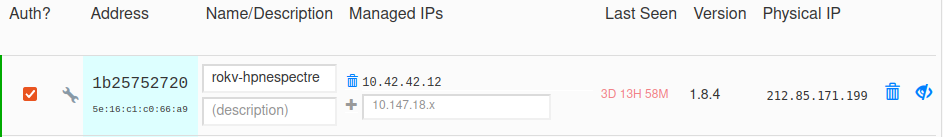
\includegraphics[width=1\textwidth]{fotografije/administering_ZeroTier.png}
\end{center}
\caption{Pregled nad enim izmed odjemalcev našega omrežja ZeroTier \cite{rvidmar}}
\label{administering_ZeroTier}
\end{figure}

\subsection{Izvajanje omrežnih pravil na VL2}
Rešitev omogoča funkcionalnosti virtualnega omrežnega stikala. Nad odjemalci lahko izvajamo akcije, prikazane v tabeli \ref{tabela_zt_akcije}, ki jih izvajamo na nivoju VL2. Nekatere spremembe, ki jih naredimo, so na omrežju vidne v roku minute. Če imamo nastavitev, ki obravnava določenega odjemalca in je ta trenutno priključen na omrežje, bo moral znova vzpostaviti povezavo, da bodo nastavitve prišle v veljavo. S pomočjo različnih pravil lahko z rešitvijo ZeroTier dobimo funkcionalnosti upravljanega stikala L2 na navideznem zasebnem omrežju. Ekvivalent navideznega omrežja LAN (angl. Virtual LAN --- VLAN) je, da vzpostavimo več vzporednih omrežji ZeroTier.%managed ethernet switch
%dopiši o možnosti VLAN-ov

\begin{table}[H]
\begin{center}
\noindent\begin{tabular}{p{0.2\textwidth}|p{.7\textwidth}}
akcija & {\tt opis}\\ \hline
{\tt drop} & opusti okvir \\
{\tt accept}   & sprejmi okvir \\
{\tt redirect} & preusmeri okvir \\
{\tt tee}   & opazuj in posreduj okvir \\
{\tt watch} & opazuj in posreduj okvir (kot tee, le da opusti okvirje, če ni opazovalca) \\
\end{tabular}
\end{center}
\caption{Možne akcije v omrežju ZeroTier}
\label{tabela_zt_akcije}
\end{table}
\subsection{Programsko definirano prostrano omrežje - izpad}
ZeroTier v svoji dokumentaciji opisuje tudi možnosti za večpotje (angl. Multipath). Pri tem testu smo uporabili robni usmerjevalnik, opisan v poglavju \ref{implementacija_usmerjevalnika}. ZeroTier lahko v temu primeru uporablja različne nastavitve za preklop internetnega dostopa. V svoji konfiguraciji omogoča različne politike za usmerjanje prometa, ki se zgledujejo po politikah, ki so vgrajene tudi v sistem Linux. To so razpršeno oddajanje (angl. broadcast), aktivna rezerva (angl. active backup), uravnoteženo krožno dodeljevanje (angl. balanced round robin) ali uravnotežen XOR.

Za vrednotenje te funkcionalnosti smo načrtovali test; izmerili smo koliko paketov ICMP ping se izgubi od trenutka, ko je aktivna povezava prekinjena, do trenutka, ko se vzpostavi preko redundantne povezave. Tako smo izmerili, za kolikšen čas se je izgubila povezava do pisarne.

%To test smo naredili s tremi različnimi konfiguracijami. Najprej smo vzpostavili kontrolni rezultat brez posebne ZeroTier konfiguracije, potem pa smo naredili še enak test z konfiguracijo “Aktivna rezerva” ter “Razpršena oddaja”.

\begin{figure}[h]
\begin{center}
\includesvg[width=1\textwidth]{fotografije/SDWAN_test_arhitektura(1).svg}
\end{center}
\caption{Shema testne metodologije za izpad fiksnega dostopa \cite{rvidmar}}
\label{izpad_dostopa}
\end{figure}

Pri testiranju izpada primarne povezave v omrežju ZeroTier smo prišli do težav. Konfiguracija za aktivno redundanco do omrežja VPN ni ustrezno delovala. Odjemalec ZeroTier po izpadu primarne povezave ni avtomatsko poiskal nove poti do strežnikov in soležnikov.
To se je zgodilo, kljub temu da je preklop naše povezave na sekundarni dostop v internet s pomočjo programskega paketa MWAN3 (opisano v poglavju \ref{MWAN3}) na platformi OpenWRT deloval in na usmerjevalniku nismo izgubili povezave do interneta. Med izgubo primarne povezave ni trajalo več kot 3 sekunde, da je bil promet preusmerjen na sekundarno povezavo WAN prek omrežja LTE/NR. Težava je, da ostali soležniki na sekundarni povezavi ne bodo videli omrežja za usmerjevalnikom. Uporabniki lokalnega omrežja bodo lahko dostopali do interneta, vendar ne do soležnikov omrežja ZeroTier. Če se primarna povezava vrne, se vzpostavi nazaj tudi omrežje ZeroTier.

Težavo, da ZeroTier ne vzpostavi nove poti do soležnikov, smo poskušali rešiti tudi s funkcionalnostjo, ki jo ponuja MWAN3, in sicer da ob izpadu kliče skripto v programskem jeziku "bash". V skripto smo napisali, da se storitev ZeroTier na robnem usmerjevalniku 5 sekund po izpadu znova zažene, ko ima že povezavo prek javnega naslova mobilnega omrežja, vendar se poti kljub temu ne vzpostavijo same. Za aplikacijo, ki smo si jo zamislili, bi rešitev ZeroTier v tem primeru odpovedala.

\subsection{Zagotavljanje kakovosti storitev}
V dokumentaciji ZeroTier \cite{noauthor_protocol_nodate} so opisani mehanizmi zagotavljanje storitev; storitve kvalificiramo v 9 različnih razredov prioritete glede na vrata transportnega nivoja UDP ali TCP. Primer: prioritiziramo komunikacijo VoIP na določenih vratih UDP pred ostalim prometom, da ostane komunikacija nemotena, kjub temu da vzporedno prenašamo velike datoteke.

Za vrednotenje lastnosti smo načrtovali test. Skozi VPN peljemo dva prometna tokova z orodjem "iPerf3", ki za povezavo na transportnem nivoju uporabljata druga vrata, prikaz arhitekture testa na sliki \ref{qos_shema}. Najprej bomo test opravili brez vsakršnih nastavitev za zagotavljanje kakovosti storitev, kot kontrolo. V naslednji iteraciji testa bomo enemu podatkovnemu toku nastavili višjo prioriteto kot drugemu ter opazovali, ali pride do spremembe v hitrostih v primerjavi s kontrolnim testom.

%https://iperf.fr/iperf-download.php
\begin{figure}[h]
\begin{center}
\includesvg[width=1\textwidth]{fotografije/qos_test(1).svg}
\end{center}
\caption{Shema testne metodologije za funkcijo zagotavljanje kakovosti storitve \cite{rvidmar}}
\label{qos_shema}
\end{figure}
Pri konfiguraciji zagotavljanja kakovosti omrežja smo prav tako našli pomanjkljivosti v dokumentaciji. Medtem ko so v beli knjigi (angl. white paper) tehnologije ZeroTier mehanizmi za zagotavljanje kakovosti storitev opisani, jih v bolj podrobni dokumentaciji ni mogoče najti. Po raziskavi dokumentacije in uradnih spletnih forumov rešitve ZeroTier smo ugotovili, da ta funkcionalnost ni implementirana, kljub temu da je opisana v beli knjigi. Načrtovanega testa za vrednotenje te lastnosti nismo mogli izvesti.

\section{Implementacija omrežja ZeroTier}
ZeroTier omrežje smo implementirali po spodaj nevedenem scenariju; ker trenutne razmere ne dopuščajo, da vsi zaposleni delajo iz pisarne, delajo oddaljeno od doma. V podjetju se nahaja strežnik s pomembnimi datotekami, do katerih morajo zaposleni dostopati. Zato smo v podjetju nastavili robni usmerjevalnik, na katerem teče odjemalec ZeroTier ter usmerja promet v lokalno omrežje v pisarni. Ker mora biti delo nemoteno, smo v pisarni nastavili redundančni dostop do interneta. Tako ima robni usmerjevalnik dostop do interneta prek koaksialnega kabla pri enem operaterju ter prek 5G NR mobilnega omrežja redundančni dostop, na katerega se promet ob potencialnem izpadu preusmeri. Načrtovano omrežje na sliki \ref{shema_realizacije}.

\begin{figure}[h]
\begin{center}
\includesvg[width=1\textwidth]{fotografije/Implementacija_scenarji_1.svg}
\end{center}
\caption{Shema omrežja, ki smo ga realizirali \cite{rvidmar}}
\label{shema_realizacije}
\end{figure}

\section{Implementacija rešitve ZeroTier na usmerjevalniku}
\label{implementacija_usmerjevalnika}
%se dodaj en odstavek
Rešitev ZeroTier omogoča implementacijo na usmerjevalnikih --- podprt je na širokem spektru platform, med drugimi tudi na usmerjevalniških platformah, kot  sta OpenWRT \cite{brown_welcome_2016} ter RouterOS \cite{noauthor_mikrotik_nodate}. %http://www.mikrotik-routeros.net/routeros.aspx

\subsection{Izbira strojne opreme}

Pri implementaciji smo se odločili za strojno platformo Raspberry Pi 4 (v nadaljevanju RPi), saj za svojo ceno ponuja veliko fleksibilnost ter zmogljivost. Procesorska moč je pomembna, saj bo naš robni usmerjevalnik šifriral promet, ki se bo pretakal po VPN-ju. Slabost uporabe platforme RPi za aplikacijo usmerjevalnika je, da ima premalo vmesnikov Ethernet. Da ga uporabimo kot usmerjevalnik, potrebujemo vsaj dva takšna vmesnika, enega za internet ter drugega za lokalno omrežje. To smo rešili s prilagodilnikom, ki nam pretvori USB 3.0 vhod v gigabitni ethernet (USB omrežni krmilnik --- NIC), slika \ref{robni_usmerjevalnik}. RPi tako opravlja nalogo prehodnega usmerjevalnika ter požarne pregrade.

Alternativna izbira za našo implementacijo bi bila usmerjevalnik znamke MikroTik, baziran na arhitekturi ARM, ki ima prav tako podporo za odjemalca ZeroTier. MikroTik uporablja operacijski sistem RouterOS, ki je zelo fleksibilna platforma za usmerjevalnike. RouterOS prav tako bazira na jedru Linux.

\begin{figure}[h]
\begin{center}
\includesvg[width=0.8\textwidth]{fotografije/RPI_robni_usmerjevalnik.svg}
\end{center}
\caption{Shema usmerjevalnika RPi, ki služi kot prehod v internet. \cite{rvidmar}}
\label{robni_usmerjevalnik}
\end{figure}

\subsection{Izbira programske opreme}
Za programsko opremo smo izbrali OpenWRT \cite{brown_welcome_2016}. To je operacijski sistem, ki bazira na Linuxu. Njegove funkcionalnosti so prilagojene prav za aplikacije, kot je naša --- usmerjevalnik. Prilagojen je za enostavno konfiguracijo usmerjevalnika internetnega prometa na vgradnih sistemih. Za projektom OpenWRT je tudi velika odprtokodna skupnost, ki operacijski sistem nenehno popravlja in nadgrajuje. Prednost OpenWRT-ja je tudi v tem, da ima veliko razširitev, ki lahko vgradnim platformam razširi funkcionalnost. Pri naši implementaciji smo uporabili kar nekaj paketov, kot so: goniniki za omrežni vmesnik USB, odjemalec za ZeroTier VPN, spletni uporabniški vmesnik za upravljanje z RPi.

\subsection{Konfiguracija OpenWRT na RPi}
RPi smo konfigurirali kot usmerjevalnik in požarno pregrado, da lahko služi kot prehodni usmerjevalnik v internet in podpira gigabitne hitrosti. Za to, da je vmesnik iz USB v Ethernet ustrezno deloval, smo morali najti ustrezni gonilnik. OpenWRT ima dobro podporo gonilnikov za vmesnike USB-Ethernet. Vmesnike smo ustrezno konfigurirali, tako da en vmesnik povezuje stran LAN in drug vmesnik stran WAN, kar je prikazano na sliki \ref{OpenWRTconfig}. Na strani LAN teče tudi strežnik DHCP, ki deli naslove IP na strani LAN. Na sistem OpenWRT smo naložili tudi paket za spletni uporabniški vmesnik LuCI (angl. Lua programming language, configuration interface) \cite{noauthor_luci_nodate}. Ta nam omogoči, da sistem OpenWRT konfiguriramo tudi prek spletnega uporabniškega vmesnika. LuCI uporabniku, ki ni spreten v ukazni vrstici, uporabo sistema OpenWRT poenostavi. LuCI ponuja več funkcionalnosti, kot jo najdemo na spletnih uporabniških vmesnikih potrošniških usmerjevalnikov. Nudi tudi dober pregled nad sistemskimi viri, utilizacijo ter pregled nad prometom po posameznih vmesnikih.

\begin{figure}[h]
\begin{center}
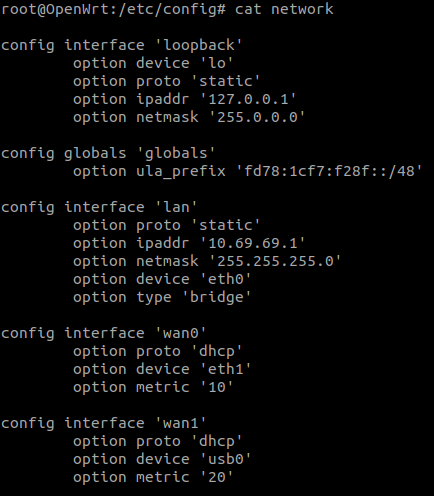
\includegraphics[width=0.6\textwidth]{fotografije/openWRTconfig.png}
\end{center}
\caption{Konfiguracija vmesnikov v okolju OpenWRT \cite{rvidmar}}
\label{OpenWRTconfig}
\end{figure}

\subsection{MWAN3 za aktivno redundanco internetnega dostopa}
\label {MWAN3}
MWAN3 je paket za platformo OpenWRT, ki doda funkcionalnosti, ki jih potrebujemo če imamo več povezav v prostrano omrežje \cite{dyck_mwan3_2013}. Omogoča uravnovešeno pošiljanje prometa po več povezah WAN ali da se povezave preusmerijo na drug vmesnik WAN v primeru odpovedi internetne povezave na prvem vmesniku. MWAN3 omogoča tudi usmerjanje na podlagi politike (angl. Policy Based Routing --- PBR). Politike se lahko nastavljajo na podlagi vrat, naslovov IP itd. Orodje MWAN3 ima tudi možnost, da nas ob izpadu dostopa do interneta na vmesniku opozori, tako da zažene skripto v programskem jeziku "bash", ki jo lahko sami poljubno urejamo, npr. lahko bi nam poslala e-pošto.

V našem primeru smo MWAN3 konfigurirali v način, da je bila povezava prek fiksnega internetnega dostopa primarna, povezava prek modema za mobilno omrežje pa sekundarna. To smo dosegli s pomočjo dodelitve metrik posameznim vmesnikom WAN. Manjša kot je metrika, bolj pomembna je povezava. V našem primeru smo  fiksni povezavi do interneta prek koaksialnega kabla določili metriko ena, sekundarni povezavi prek mobilnega omrežja pa metriko dve. To konfiguracijo smo tudi testirali in prišli do rezultatov, da traja izpad omrežja, ko prestavimo iz primarnega na sekundarno omrežje, 5---10 sekund; v obratno smer izpad ni opazen. Izpad dostopa do interneta smo opazovali in izmerili s pomočjo ukaza, ki nam vrne naš javni naslov IP, ki se izvaja 4-krat na sekundo.
Izpad smo izmerili z naslednjim ukazom v okolju Linux:

\begin{code}

\begin{minted}{bash}
    $ while sleep 0.2; do dig +short \
    myip.opendns.com @resolver1.opendns.com| ts; done
    

\end{minted}
\captionof{listing}{Ukaz za izpis javnega naslova v while zanki.}
\label{command_publicIP}

\end{code}
\hspace{1cm}

Spodaj lahko vidimo primer prehoda iz fiksnega omrežja na mobilno, ki se je zgodil v šestih sekundah:

\begin{code}
\begin{minted}{bash}

    ...
    Feb 14 22:10:40 31.15.134.41
    Feb 14 22:10:40 31.15.134.41
    Feb 14 22:10:46 188.197.0.76
    Feb 14 22:10:46 188.197.0.76
    Feb 14 22:10:47 188.197.0.76...

\end{minted}
\captionof{listing}{Izvleček izpisa ukaza \ref{command_publicIP}, kjer lahko vidimo prehod med dvema različnima javnima naslovoma (fiksni dostop, ter 5G NR).}
\end{code}
\hspace{1cm}
\chapter{Metodologija vrednotenja rešitev VPN}
\label{methodology}

%----------------------------------------------
\begin{comment} %to je romalo v sekcijo ZeroTier pod programsko definirana omrežja
Za vrednotenje rešitve smo načrtovali več različnih testov, ki so nam pomagali objektivno oceniti rešitev. ZeroTier omogoča nekaj funkcij programsko definiranega omrežja, ki niso predvsem konvencionalne za VPN. Omogoča, da imamo na kontrolni ravnini nadzor nad odjemalci, ter njihovim naslovi, ima pa tudi mehanizme za funkcije programsko definiranega prostranega omrežja, in sicer različne politike za redundanco, ter funkcije za zagotavljanje kakovosti storitev. Za vrednotenje teh funkcij smo izvedli tri teste:
\begin{itemize}
    \setlength\itemsep{0em}
    \item Upravljanje s klienti s kontrolne ravnine,
    \item kako delujejo različne politike za redundanco,
    
    \item kako delujejo mehanizmi za zagotavljanje kvalitete storitev.
\end{itemize}
\end{comment}
%-----------------------------------------------


ZeroTier smo primerjali z drugimi konkurenčnimi odprtokodnimi rešitvami.  Za konkurenčne rešitve smo izbrali:
\begin{itemize}
    \setlength\itemsep{0em}
    \item OpenVPN, ki je predstavnik rešitev, ki temeljijo na protokolu TLS/SSL,
    
    \item IKEv2/IPSec, ki predstavlja najbolj varen in učinkovit protokol, ki temelji na IPSec,
    
    \item WireGuard, ki predstavlja novejšo konkurenčno rešitev na aplikacijskem nivoju.
\end{itemize}

Primerjali smo zahtevnosti administracije rešitev z vidika sistemskega administratorja, in sicer kako težko je vzpostaviti same strežnike VPN ter kako zahtevno je vršiti administracijo nad samimi uporabniki.
Primerjali smo tudi pretočnost omenjenih rešitev za vzpostavljanje omrežji VPN ter kako odporna je posamezna rešitev na prehajanje med različnimi dostopi.
Za vrednotenje omenjenih lastnosti smo načrtovali štiri teste:
\begin{enumerate}
    \item ocena težavnosti integracije, poglavje \ref{test_integracija},
    \item ocena funkcij administracije omrežja VPN, poglavje \ref{test_administracija},
    \item učinkovitost rešitev (pretočnost), poglavje \ref{test_ucinkovitost},
    \item stabilnost povezave do omrežja VPN med prehajanjem (Wi-Fi - mobilno omrežje), poglavje \ref{test_stabilnost}.
\end{enumerate}

Za potrebe testiranja smo implementirali strežnik (krmilnik v primeru ZeroTier) ter odjemalca na sistemu Linux in Android za vsako od rešitev, prikazano na sliki \ref{implementacija}. Strežnike/krmilnike za vse rešitve smo integrirali na operacijskem sistemu Linux Ubuntu 20.04 LTS. Odjemalce smo konfigurirali na operacijskih sistemih Linux Raspbian (posebej prilagojena distribucija Linux Debian za sisteme Raspberry Pi) in na sistemu Android 12 (naprava Google Pixel 6).

\begin{figure}[h]
\begin{center}
\includesvg[width=1\textwidth]{fotografije/testing_environment (1)(1)(1).svg}
\end{center}
\caption{Arhitektura omrežja, ki smo ga realizirali za vse rešitve VPN. \cite{rvidmar}}
\label{implementacija}
\end{figure}

\section{Težavnost integracije}
\label{test_integracija}
Med postopkom namestitve smo ugotovili, kako težko je vsako rešitev implementirati. Tako smo lahko ocenili zahtevnost vsake implementacije od ena do tri. Ocena ena pomeni, da lahko omrežje vzpostavi tehnično podkovan uporabnik računalnika, ocena tri pomeni, da mora imeti integrator rešitve dobro poznavanje okolja Linux in omrežne tehnologije.

\section{Administracija --- upravljanje omrežja}
\label{test_administracija}
Pri administraciji smo ocenili, kakšne možnosti ponuja rešitev za pregled nad uporabniki. V oceno smo vključili tudi to, kako zahtevno je vršiti operacije nad uporabniki. Za vrednotenje smo prav tako kot pri integraciji uporabili ocene od ena do tri, kjer ocena ena pomeni, da rešitev nima veliko funkcij in ni primerna za uporabo v poslovne namene, tri pa, da ima rešitev dobro realiziran pregled nad uporabniki ter da je primerna tudi za poslovno uporabo.



\section{Učinkovitost navideznega zasebnega omrežja --- pretočnost}
\label{test_ucinkovitost}
Učinkovitost rešitev VPN smo testirali tako, da smo izmerili maksimalno pretočnost pri omejenih računskih virih. Za potrebe testiranja učinkovitosti smo vzpostavili testno okolje, kjer smo omejili računsko zmogljivost odjemalca zato, da vidimo, kakšna je učinkovitost šifriranja in protokola VPN. Vire smo omejili tako, da je eden od odjemalcev Raspberry 3B+, ki ima omejeno računsko moč za šifriranje internetnih hitrosti, ki jih dosegamo danes. Opazovali smo pretočnost med odjemalcem in strežnikom, saj pri slabše optimiziranih rešitvah VPN pretočnost pade. Pretočnost smo izmerili z odprtokodnim orodjem iPerf3, ki se uporablja za merjenje hitrosti v omrežjih.

Testno okolje sestavlja strežnik za VPN, na katerega se poveže odjemalec VPN, prikazano na sliki \ref{throughput}. Strežnik ima dostop v omrežje s hitrostjo 600 Mbit/s v smeri proti strežniku in 60 Mbit/s v smeri interneta. Na drugem dostopu je odjemalec VPN RPi, ki ima hitrost proti odjemalcu 750 Mbit/s, v smeri proti internetu pa 150 Mbit/s. Pretok smo merili v smeri od odjemalca proti strežniku, kot je prikazano na sliki \ref{throughput}. V to smer smo bili omejeni z 150 Mbit/s, kar se je izkazalo za dovolj veliko hitrost, da je pretočnost omejeval RPi.

Uporabili smo naslednji iPerf3 ukaz, ki ustvari pet podatkovnih tokov TCP in ustvarja promet pet minut v smeri od strežnika proti odjemalcu, podatke izpisuje v obliki JSON za nadaljno obdelavo:

\begin{minted}{bash}
    $ iperf3 -c 10.10.10.24 -P 5 -t 300 -J -R
  
\end{minted}

\begin{figure}[h]
\begin{center}
\includesvg[width=0.6\textwidth]{fotografije/performance_setup(1).svg}
\end{center}
\caption{Shema testne metodologije za testiranje učinkovitosti in pretočnosti izbranih rešitev VPN \cite{rvidmar}}
\label{throughput}
\end{figure}


\section{Stabilnost povezave med menjavanjem internetnega dostopa odjemalca}
\label{test_stabilnost}
V nekaterih primerih hočemo biti na VPN povezani vedno, tudi v primeru, ko na mobilni napravi preidemo iz mobilnega na Wi-Fi omrežje ali obratno. V tem testu smo testirali, kaj se zgodi s povezavo VPN, ko mobilno napravo prestavimo iz Wi-Fi na mobilno omrežje, prikazano na sliki \ref{roaming}. Ali se prekine? Za koliko časa se prekine? S pomočjo orodja “Ping” smo izmerili, za koliko časa se je povezava do VPN izgubila in ali se je avtomatsko vzpostavila nazaj. Za interval paketov ping smo izbrali 0,2 sekunde, kar nam omogoči ustrezno granulacijo za evalvacijo prekinitve. Aplikacije za videoklice ter VoIP delujejo dobro, dokler je izguba povezave krajša od 0,3 sekunde. Če izgubimo povezavo za več kot 0,3, uporabnik občuti opazno degradacijo - zamrznitev slike/izgubljanje besed. Naš ključni kazalnik uspešnosti (angl. Key performance indicator - KPI) bo, da je povprečje petih meritev prehoda omrežja manjše od 0,3 sekunde.

Meritev smo ločili na prehod iz lokalnega omrežja Wi-Fi na mobilno omrežje in obratno. V vsako smer smo naredili 5 meritev in rezultat povprečili.

\begin{figure}[h!]
\begin{center}
\includesvg[width=0.8\textwidth]{fotografije/test_prehajanje.svg}
\end{center}
\caption{Shema testne metodologije za testiranje prehajanja med omrežji \cite{rvidmar}}
\label{roaming}
\end{figure}

Na strežniku VPN smo uporabili spodnji ukaz v okolju Linux. Argument -i določi interval poslanih paketov ping v sekundah. Argument -O pa nam omogoči, da v ukazni vrstici vidimo tudi pakete, ki so se izgubili ali pa se niso še vrnili v času intervala paketov ping. Ukaz Linux:
\begin{minted}{bash}
  $ ping 10.10.100.1 -O -i 0,2
\end{minted}




%rezultati
\chapter{Rezultati testiranja rešitev VPN}
\label{rezultati}
\section{Težavnost integracije}
\subsection{ZeroTier}
Za delovanje rešitve ZeroTier moramo vnesti samo nekaj ukazov v ukazni vrstici in rešitev deluje. Za uporabniški vmesnik krmilnika ZeroTier smo uporabili odprtokodno rešitev, ki jo je razvila ekipa KeyNetworks, ZTNCUI --- ZeroTier network controller user interface \cite{noauthor_key_nodate}.

Najprej smo naložili ZeroTier aplikacijo na platformi Linux Ubuntu z ukazom:
\begin{minted}{bash}
$ curl -s https://install.ZeroTier.com | sudo bash
\end{minted}

Prenesli in naložili smo instalacijsko datoteko za ZTNCUI \cite{noauthor_key_nodate} z ukazi:
\begin{minted}{bash}
$ curl povezava_do_instalacjiske_datoteke/ztncui_0.8.6_amd64.deb
$ sudo apt-get install ./ztncui_0.8.6_amd64.deb
\end{minted}

Če postavljamo krmilnik na javnem naslovu IP, moramo ustrezno poskrbeti za varnost pred napadi iz javnega omrežja. Mi smo rešitev postavili znotraj lokalnega omrežja in imeli požarni zid nastavljen na prehodnem usmerjevalniku.
Za delovanje potrebujemo nastaviti še vrata TCP za spletni uporabniški vmesnik:
\begin{minted}{bash}
$ sudo sh -c "echo 'HTTPS_PORT=3443' > /opt/key-networks/ztncui/.env"
\end{minted}

Potem samo še ponovno zaženemo aplikacijo ZeroTier z ukazom:
\begin{minted}{bash}
$ sudo systemctl restart ztncui
\end{minted}

Sedaj je uporabniški vmesnik za ZeroTier omrežje na voljo na povezavi "https://localhost:3443'' z računalnika, kjer je naložen uporabniški vmesnik (lahko tudi z drugega računalnika na istem omrežju, kjer "localhost'' nadomestimo z IP-naslovom računalnika, kjer se nahaja krmilnik), prva stran spletnega uporabniškega vmesnika na sliki \ref{ZeroTier_UI}. Cela namestitev je zelo enostavna, potrebujemo samo zgoraj navedene ukaze in smo že pripravljeni, da lahko na omrežje povežemo prve odjemalce.

ZeroTier ponuja tudi gostovanje krmilnika ZeroTier na njihovi spletni strani. Ko imamo uporabniški račun na njihovi spletni strani, lahko naredimo novo omrežje ZeroTier z enim klikom. To nikakor ni varna ali zanesljiva rešitev VPN, je pa uporabniku prijazna.


\begin{figure}[h]
\begin{center}
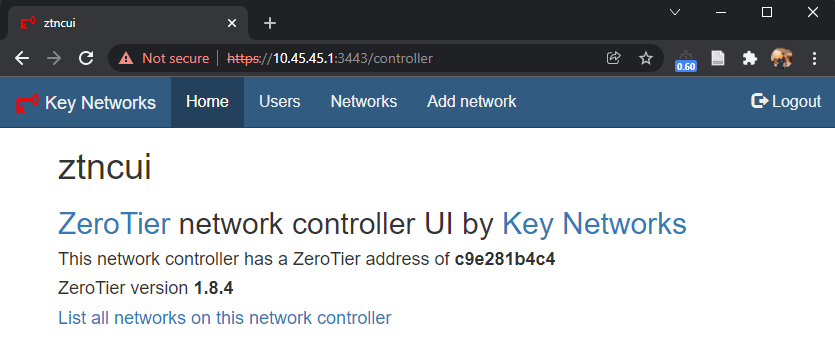
\includegraphics[width=1\textwidth]{fotografije/ztncui_posnetek zaslona.png}
\end{center}
\caption{Prva stran uporabniškega vmesnika za krmilnik ZeroTier \cite{rvidmar}}
\label{ZeroTier_UI}
\end{figure}

\subsection{OpenVPN}

Rešitev OpenVPN ponuja širok spekter nastavitev. Mi smo pri implementaciji uporabili privzete nastavitve. Če imamo posebne zahteve za našo konfiguracijo, OpenVPN to ponuja, vendar je namestitev potem bolj zahtevna.

Za namestitev rešitve OpenVPN je odprtokodna skupnost naredila skripto, ki nastavitev strežnika za OpenVPN zelo olajša. Najdemo jo lahko na "https://git.io/vpn" (17.3.2022). Skripto prenesemo in zaženemo na platformi Linux Ubuntu s pomočjo ukazov:
\begin{minted}{bash}
$ wget https://git.io/vpn -O openvpn-install.sh #prenos
$ sudo bash openvpn-install.sh #zagon
\end{minted}

Ta nas vodi skozi namestitveni postopek in nam pomaga kreirati uporabniški profil za povezavo na strežnik, namestitveni postopek prikazan na sliki \ref{Namestitev_OpenVPN}. Uporabniški profil se nam izvozi v obliki datoteke ".ovpn", ki jo lahko uvozimo v odjemalca za OpenVPN na kateri koli napravi, ki jo rešitev OpenVPN podpira. Več uporabniških profilov lahko dodamo tako, da še enkrat zaženemo to skripto.

V našem primeru imamo strežnik OpenVPN na zasebnem naslovu IP za prehodnim usmerjevalnikom. Da se lahko odjemalci povežejo na naš strežnik, moramo zato dodati ustrezna pravila NAT. Za OpenVPN je razvit spletni uporabniški vmesnik za bolj prijazno uporabo pod imenom OpenVPN Access Server.

\begin{figure}[H]
\begin{center}
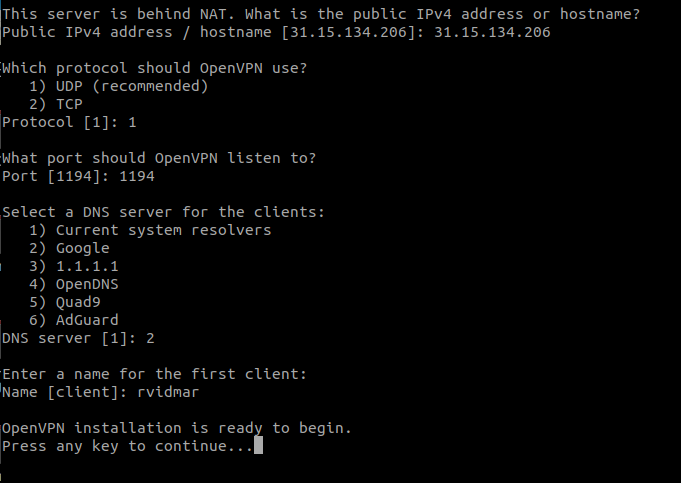
\includegraphics[width=0.8\textwidth]{fotografije/nalaganjeOvpn.png}
\end{center}
\caption{Namestitev strežnika OpenVPN s pomočjo skripte \cite{rvidmar}}
\label{Namestitev_OpenVPN}
\end{figure}

\subsection{WireGuard} %cite wireguard quickstart reference https://www.wireguard.com/quickstart/
Namestitev rešitve WireGuard je nekoliko bolj zahtevna od rešitve ZeroTier \cite{donenfeld_quick_nodate}. Od nas zahteva da sami generiramo zasebne in javne ključe za avtentikacijo. Najprej moramo WireGuard namestiti na sistem Linux Ubuntu, to naredimo z ukazom:

\begin{minted}{bash}
$ sudo apt install wireguard
\end{minted}

Za delovanje WireGuard-a moramo generirati zasebni in javni ključ, ki je izračunan iz zasebnega. Najlažje to naredimo z ukazom:

\begin{minted}{bash}
$ wg genkey | tee privatekey | wg pubkey > publickey
\end{minted}

Naredimo ustrezen omrežni vmesnik za omrežje VPN "wg0'' z željenim podomrežjem (v našem primeru 192.168.6.1/24) z ukazom:
\begin{minted}{bash}
$ ip address add dev wg0 192.168.6.1/24
\end{minted}
 
Za delovanje moramo ustrezno urediti konfiguracijsko datoteko, ki se v Linux nahaja v direktoriju ''/etc/wireguard/wg0.conf", prikazano na sliki \ref{wireguard_conf}. Lahko opazimo, da smo pod značko "[Peer]" že vnesli javne ključe za povezavo odjemalcev. Po podobnem zgledu naredimo tudi konfiguracijsko datoteko za odjemalca. Več o nastavitvah odjemalcev v poglavju \ref{Rezultati_Administracija}.

Na prehodnem usmerjevalniku smo odprli tudi ustrezna vrata UDP (kot vidimo na konfiguracjiski datoteki na sliki \ref{wireguard_conf}, v našem primeru vrata UDP 40002)

\begin{figure}[h]
\begin{center}
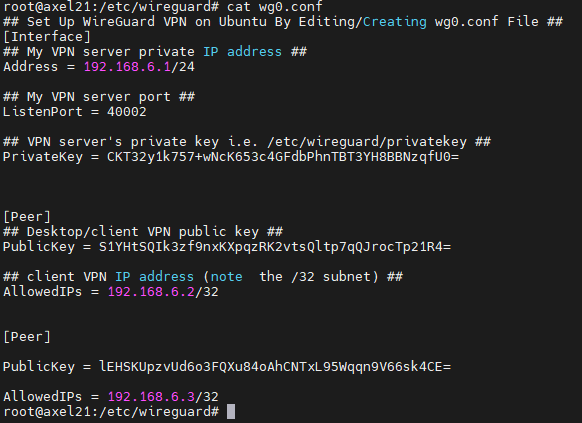
\includegraphics[width=0.8\textwidth]{fotografije/WireGuard_Config_file_server.png}
\end{center}
\caption{Konfiguracijska datoteka za omrežje WireGuard \cite{rvidmar}}
\label{wireguard_conf}
\end{figure}

\subsection{IKEv2/IPSec} %reference digital ocean tutorial

Pri implementaciji IKEv2/IPSec smo si pomagali z rešitvijo ''StrongSwan" \cite{noauthor_strongswan_nodate}. ''StrongSwan" je odprtokodna rešitev, ki omogoča uporabo protokola IKEv2/IPSec. Sama implementacija je zahtevnejša od ostalih opisanih, zato bomo nekaj korakov samo na kratko opisali.
Najprej moramo naložiti vse potrebne pakete, ki so potrebni poleg aplikacije StrongSwan, z ukazom:

\begin{minted}{bash}
$ sudo apt install strongswan strongswan-pki libcharon-extra-plugins \
libcharon-extauth-plugins libstrongswan-extra-plugins
\end{minted}

Za delovanje IKEv2 smo generirali certifikate, pri tem nam pomaga aplikacija ''strongswan-pki". Potrebujemo ustrezen podpisan certifikat CA ter ustrezno podpisan certifikat strežnika. Nastavili smo še konfiguracijsko datoteko, ki se na Linux nahaja v ''/etc/ipsec.conf", vsebina datoteke, prikazana na sliki \ref{ipsec_conf}.

\begin{figure}[h]
\begin{center}
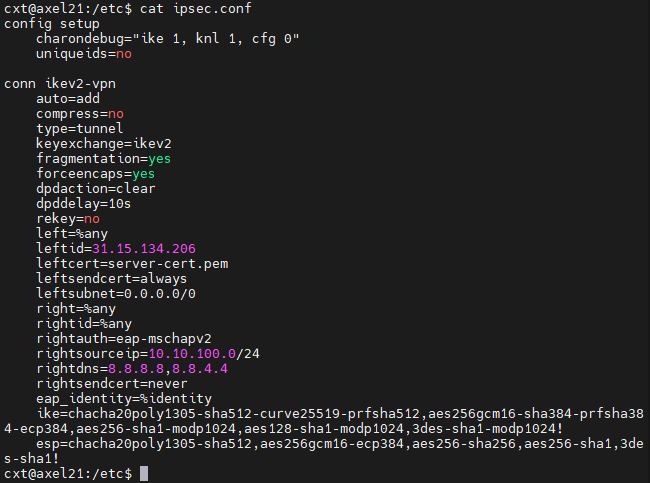
\includegraphics[width=0.8\textwidth]{fotografije/ipsec_conf.png}
\end{center}
\caption{Konfiguracijska datoteka za StrongSwan IKEv2/IPSec \cite{rvidmar}}
\label{ipsec_conf}
\end{figure}

Tako kot pri rešitvi OpenVPN ter Wireguard smo pri implementaciji IKEv2/IPSec VPN morali ustrezno skonfigurirati pravila NAT na prehodnem usmerjevalniku.

\subsection{Vrednotenje}
Vse prej opisane implementacije smo izvedli sami s pomočjo priročnikov, dostopnih na internetu \cite{tholstorf_ZeroTier_nodate,jan_just_keijser_openvpn_2017,noauthor_how_nodate-1,donenfeld_quick_nodate,noauthor_how_nodate}. Težavnost implementacije smo ocenili z ocenami od ena do tri, kjer ena pomeni, da bi se take implementacije lotil uporabnik, ki je spreten s sistemom Microsoft Windows, tri pa sistemski administrator z dobrim poznavanjem omrežnih tehnologij.

Najlažjo implementacijo izmed rešitev, ki smo jih testirali, ima ZeroTier. Naložiti moramo aplikacijo ZeroTier ter uporabniški vmesnik za krmilnik ZeroTier. Rešitev tudi ne potrebuje nastavljanja na robnem usmerjevalniku ali požarnem zidu. Nekoliko težja implementacija je pri rešitvah OpenVPN in WireGuard, pri katerih moramo biti dobro seznanjeni z omrežnimi tehnologijami, da jih lahko nastavimo. Moramo poznati principe požarnih zidov, vrat transportnega sloja v modelu OSI, DNS ter asimetričnih ključev v primeru rešitve WireGuard. Najtežja implementacija pa je za rešitev IKEv2/IPSec, kjer moramo poleg dobrega poznavanja omrežnih tehnologij tudi sami generirati in podpisovati digitalne certifikate. Ocene na sliki \ref{zahtevnostimplementacije}.
\begin{figure}[h]
\begin{center}
\includesvg[width=0.9\textwidth]{fotografije/implementacija_final.svg}
\end{center}
\caption{Ocena zahtevnosti implementacije posamezne rešitve, ena --- \mbox{enostavno}, tri --- zahtevno}
\label{zahtevnostimplementacije}
\end{figure}

\section{Administracija - upravljanje omrežja}
\label{Rezultati_Administracija}
Administracija zajema predvsem dodajanje, odstranjevanje ter pregled nad uporabniki našega omrežja VPN. To je pomemben del samega omrežja VPN, saj je le-to kompromitirano, če se na njem znajdejo uporabniki, ki ne bi smeli imeti dostopa do njega. Administracijo smo ocenili s perspektive sistemskega administratorja.
\subsection{ZeroTier}
Administracija omrežja ZeroTier je za administratorja pregledna in uporabniku prijazna. Nudi nam spletni uporabniški vmesnik, kjer lahko vidimo, katere naprave so na omrežju pooblaščene ter katere so trenutno dosegljive. Nadzor temelji na napravah, ne na uporabnikih, kar je lahko slabost. Vsako napravo moramo posebej avtorizirati v omrežje, da dobi naslov IP omrežja VPN. Pri vsaki napravi lahko tudi vidimo, kdaj je bila nazadnje povezana v omrežje, uporabniški vmesnik prikazan na sliki \ref{administracija_ZeroTier}. Napravi lahko tudi ročno nastavimo naslov IP, ki se spremeni, ko se naprava ponovno poveže v omrežje. Uporaba uporabniškega vmesnika je intuitivna, na težave naletimo, ko imamo večje število odjemalcev, saj je spletni vmesnik ob velikem številu odjemalcev nepregleden.

\begin{figure}[H]
\begin{center}
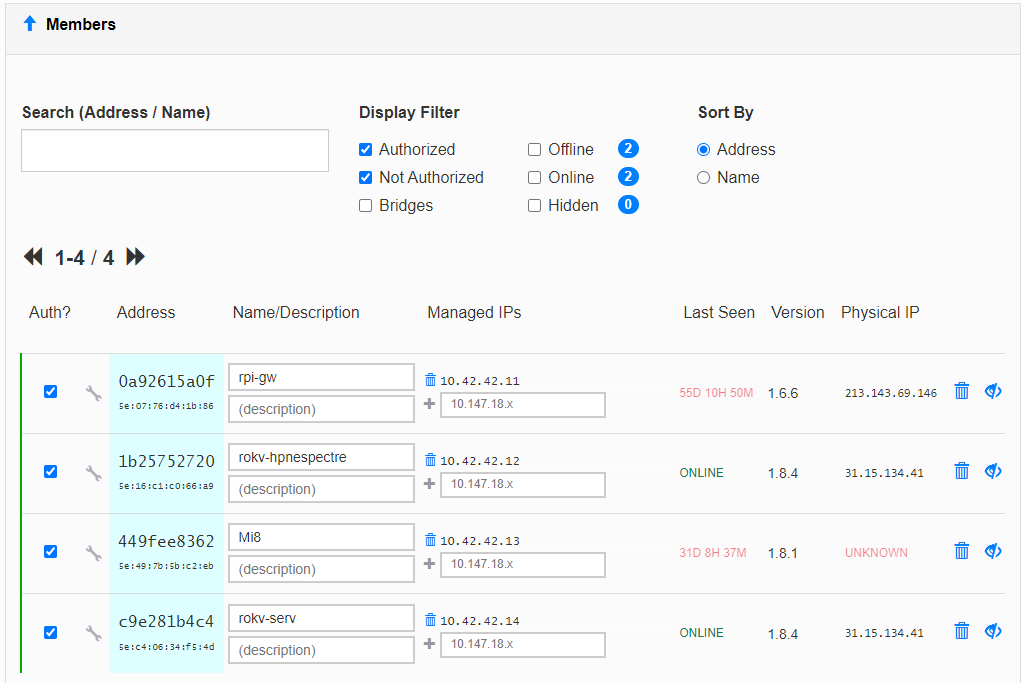
\includegraphics[width=1\textwidth]{fotografije/ZeroTier_administration.png}
\end{center}
\caption{Pregled odjemalcev omrežja ZeroTier v spletnem vmesniku \cite{rvidmar}}
\label{administracija_ZeroTier}
\end{figure}


\subsection{OpenVPN}
OpenVPN lahko v celoti kontroliramo iz ukazne vrstice, vendar pa rešitev za nadzor ponuja tudi spletni vmesnik pod imenom "OpenVPN Access Server" (v nadaljevanju OVPN-AS). V OVPN-AS lahko kreiramo uporabniške profile, slika \ref{OvpnAS_usermanagment}, s katerimi se lahko uporabniki prijavijo v OVPN-AS (to ni omrežje VPN), kjer si lahko sami ustvarijo konfiguracijske datoteke s poverilnicami za aplikacijo odjemalca VPN, s katero se uporabnik prijavi na strežnik VPN. Sama rešitev je iz administrativnega vidika zelo pregledna, imamo jasen pregled nad uporabniki. Velika prednost te rešitve je, da lahko dostop zavrnemo na nivoju uporabnika. Kot sistemski administrator lahko končnemu uporabniku damo konfiguracjisko datoteko ".ovpn", lahko pa mu damo poverilnice za OVPN-AS, kjer si konfiguracjisko datoteko kreira sam. 

\begin{figure}[h]
\begin{center}
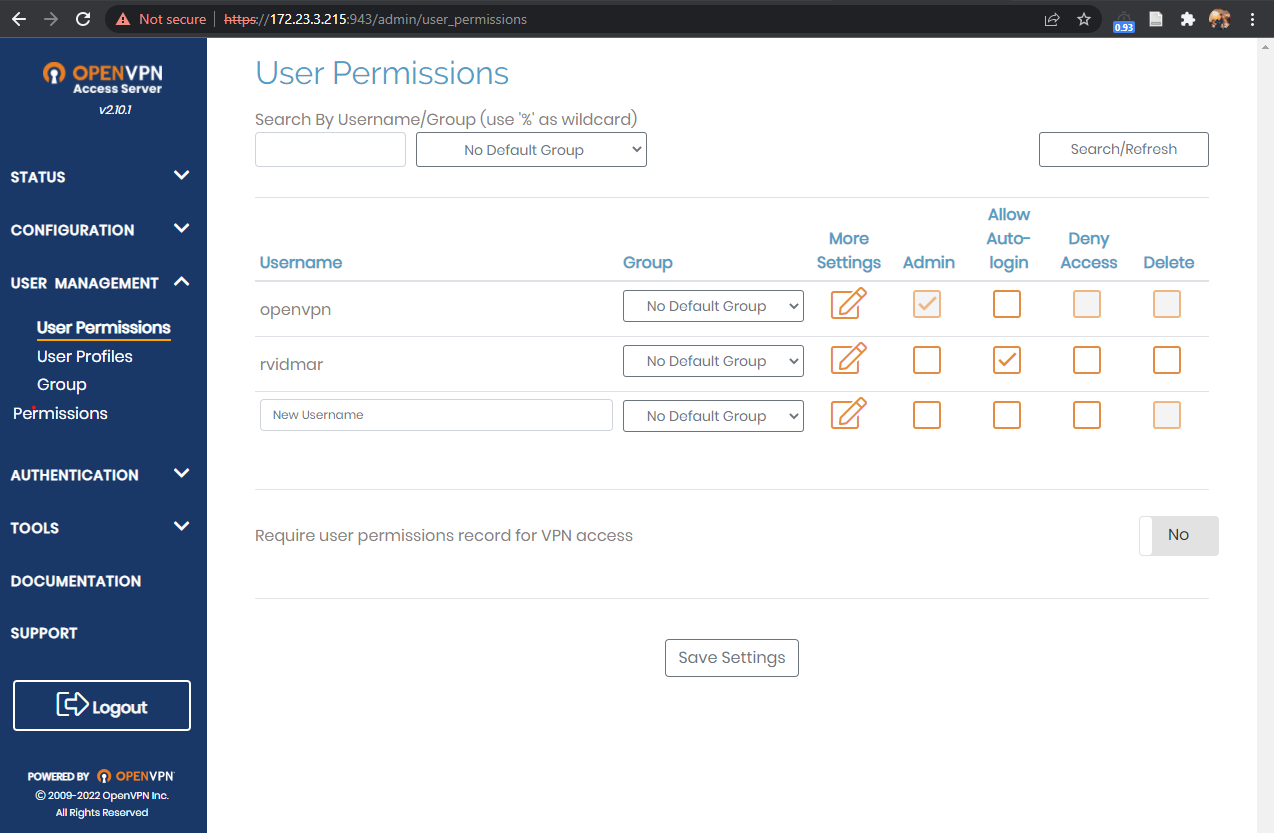
\includegraphics[width=1\textwidth]{fotografije/ovpnas_user_managment.png}
\end{center}
\caption{Zaslonski posnetek OpenVPN Access Serverja, meni, kjer lahko upravljamo med uporabniki \cite{rvidmar}}
\label{OvpnAS_usermanagment}
\end{figure}

\subsection{WireGuard}
Rešitev WireGuard ima minimalističen pristop pri svoji arhitekturi - nima uporabniškega vmesnika (več o tem v poglavju \ref{ucinkovitost_rezultati}). Administracijo opravljamo v celoti v ukazni vrstici. Avtentikacija temelji na izmenjavi javnih ključev med dvema odjemalcema --- podobno kot pri protokolu SSH. Eden od enostavnih načinov, kako izmenjati javni ključ in konfiguracjisko datoteko je, da na strežniku generiramo kodo QR ter jo poskeniramo z mobilno napravo, primer QR kode s konfiguracijo za WireGuard na sliki \ref{wg_client_qr}. Privzeto WireGuard nima nobenega mehanizma za izmenjavo teh ključev --- izmenjavo moramo opraviti prek drugega protokola, npr. SSH ali ročno. Na sliki \ref{wg_config} vidimo konfiguracijsko datoteko na strežniški. V njej najdemo javne ključe posameznih odjemalcev pod značko "Peer". Vsaka značka "Peer" predstavlja enega od odjemalcev. Vsakemu odjemalcu tukaj dodelimo naslov, ki ga bo uporabljal za navidezno zasebno omrežje.
%%Na začetku so nastavitve strežnika - določimo katero podomrežje bomo uporabili za navidezno zasebno omrežje, ter na katerih vratih strežnik posluša za nove povezave.

\begin{figure}[H]
\begin{center}

\includegraphics[width=0.7\textwidth]{fotografije/qrWG.png}
\end{center}
\caption{Konfiguracijska datoteka za odjemalca WireGuard v obliki \mbox{kode QR} \cite{rvidmar}}
\label{wg_client_qr}
\end{figure}

\begin{figure}[H]
\begin{center}
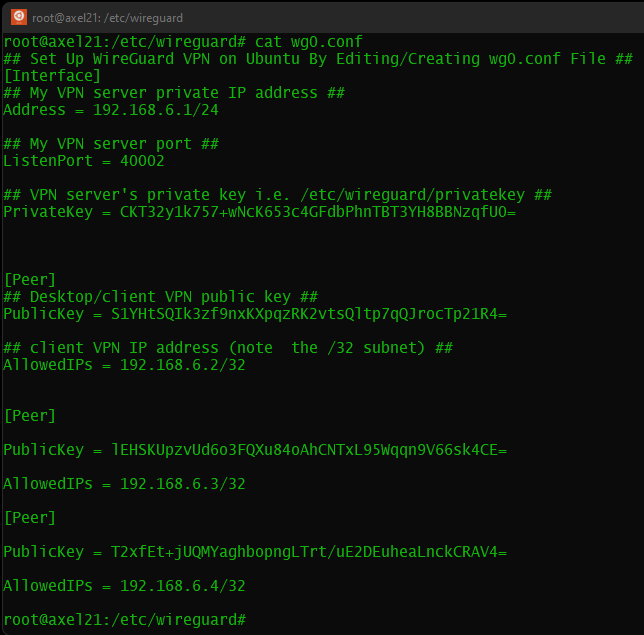
\includegraphics[width=0.7\textwidth]{fotografije/wg_config.png}
\end{center}
\caption{Konfiguracijska datoteka rešitve WireGuard na strežniški strani, v njej se nahajajo javni ključi klientov. \cite{rvidmar}}
\label{wg_config}
\end{figure}

\subsection{IKEv2/IPSec}
Administracija uporabnikov IKEv2/IPSec omrežja se vrši v ukazni vrstici. Seznam avtoriziranih uporabnikov se nahaja v "/etc/ipsec.secrets", slika datoteke \ref{ipsec_auth}. V tej datoteki imamo dober pregled nad avtoriziranimi uporabniki. Ta implementacija pa ima veliko varnostno pomanjkljivost. V primeru, da bi bil naš strežnik kompromitiran, so gesla vseh uporabnikov v obliki razumljivega besedila. To pomeni, da ni kompromitirano samo zasebno navidezno omrežje, ampak tudi gesla odjemalcev. V tej implementaciji IKEv2/IPSec, ki jo ponuja ''StrongSwan", nismo našli aktualnih orodji, ki bi omogočala dober pregled nad uporabniki omrežja VPN.

\begin{figure}[H]
\begin{center}
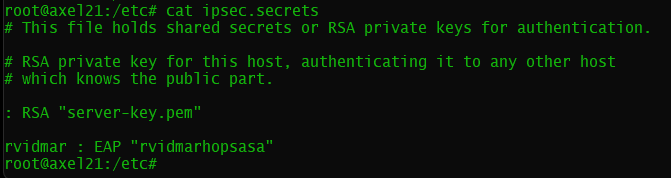
\includegraphics[width=0.7\textwidth]{fotografije/ipsec_auth.png}
\end{center}
\caption{Seznam uporabnikov, avtoriziranih v navidezno zasebno omrežje IKEv2/IPSec \cite{rvidmar}}
\label{ipsec_auth}
\end{figure}

\subsection{Vrednotenje}
Če rešitve primerjamo med sabo, slika \ref{administracija_funkcionalnost}, je za administracijo najbolj enostavna rešitev IKEv2/IPSec, saj lahko v tekstovno datoteko dodajamo in odstranjujemo uporabnike. Implementacija StrongSwan tukaj kaže veliko pomanjkljivost, saj imamo na strežniku gesla v razumljivem besedilu. Ta rešitev bi bila neprimerna za uporabo v poslovnem svetu. Najbolj fleksibilna rešitev od testiranih najbolj, ki bi bila primerna za poslovno okolje, je OpenVPN v kombinaciji z OVPN-AS. Ponuja zelo pregleden spletni uporabniški vmesnik, v katerem lahko upravljamo z uporabniki. Na njem lahko tudi nastavljamo različne načine avtentikacije. Na OVPN-AS lahko dostopajo tudi uporabniki sami, kjer si lahko generirajo konfiguracijske datoteke za odjemalsko aplikacijo.
Zelo enostaven pregled nad povezanimi napravami ima rešitev ZeroTier in ponuja tudi funkcionalnosti, kot je dodeljevanje določenih naslovov IP. Za nadzor nad napravami ima podobno funkcionalnost tudi WireGuard, vendar pregled ni mogoč v spletnem vmesniku, ampak v ukazni vrstici. Rešitvi ZeroTier ter WireGaurd se tukaj umestita med OpenVPN ter IKEv2/IPSec

\begin{figure}[H]
\begin{center}
\includesvg[width=0.9\textwidth]{fotografije/administracija_final.svg}
\end{center}
\caption{Ocena zahtevnosti administracije, ena --- neprimerno za poslovno okolje, tri --- primerno za poslovno okolje}

\label{administracija_funkcionalnost}
\end{figure}


\begin{comment}
%%%%%%%%%%%%%%%%%%%%%%
\section{Programsko definirano omrežje}
Rešitev ZeroTier ima kar nekaj funkcionalnosti programsko definiranega omrežja. Ena izmed njih je enostavna administracija nad uporabniki. V spletnem grafičnem vmesniku imamo nadzor nad vsemi povezanimi napravami, ki jim lahko nastavimo omrežne naslove. Rešitev omogoča tudi funkcionalnosti omrežnega stikala in požarne pregrade, na voljo imamo akcije vidne v tabeli \ref{tabela_zt_akcije}. Spremembe, ki jih naredimo, so na omrežju vidne zelo hitro - v roku minute. Nekatere nastavitve ne delujejo povsem v realnem času. Če imamo nastavitev, ki obravnava določenega odjemalca in je ta trenutno priključen na omrežje, bo moral znova vzpostaviti povezavo, da bojo nastavitve prišle v veljavo. S pomočjo različnih pravil lahko z rešitvijo ZeroTier dobimo funkcionalnosti upravljanega stikala L2 na navideznem zasebnem omrežju. %managed ethernet switch
%dopiši o možnosti VLAN-ov
\begin{table}
\begin{center}
\noindent\begin{tabular}{p{0.2\textwidth}|p{.7\textwidth}}
akcija & {\tt opis}\\ \hline
{\tt drop} & opusti okvir \\
{\tt accept}   & sprejmi okvir \\
{\tt redirect} & preusmeri okvir \\
{\tt tee}   & opazuj in posreduj okvir \\
{\tt watch} & opazuj in posreduj okvir (kot tee, le da opusti okvirje, če ni opazovalca) \\
\end{tabular}
\end{center}
\caption{Možne akcije v ZeroTier omrežju.}
\label{tabela_zt_akcije}
\end{table}
%%%%%%%%%%%%%%%%%%%%%%%%%%%%%%%%%%%%%%%%%%%%%%%%%
\end{comment}

\section{Učinkovitost navideznega zasebnega omrežja --- pretočnost}
\label{ucinkovitost_rezultati}

Pri testiranju učinkovitosti posameznih protokolov VPN smo prišli do ugotovitev, da rešitve OpenVPN, IKEv2/IPSec in ZeroTier dosežejo podobno pretočnost. Vsi omenjeni protokoli so pri privzetih nastavitvah omogočali pretočnost okoli 50-65Mbit/s, graf na sliki \ref{pretocnost_rpi}. Ta hitrost je bila omejena z hitrostjo enega procesorskega jedra na RPi 3B+. RPi 3B+ ne podpira strojne enkripcije, ki bi algoritme, kot so AES256 močno pohitrila. %dodaj privzete nastavitve enkripcija RPi nima podpore za hardware encryption

Vse rešitve, ki smo jih testirajo omogočajo vsaj enega od najnovejših šifrirnih algoritmov, kot so AES256, ChaCha20 in Salsa20, ki so zelo varni in učinkoviti, vendar imata tukaj protokola OpenVPN in IKEv2 težave z podporo strojnega šifriranja AES256 na različnih klientih. V tem testu se izkaže, da pri izbiri dobrega programskega šifriranja pridobimo boljšo kompatibilnost med širokim naborom naprav. AES256 je priznan varen šifrirni algoritem, ampak v primerih ko ni strojno pospešen, zelo počasen proti novejšim algoritmom kot so ChaCha20 in Salsa20 \cite{stoffelen_efficient_2019}. %reference AES CHA CHA paper for RISC 
\begin{figure}[h]
\begin{center}
\includesvg[width=0.9\textwidth]{fotografije/pretocnost_rezultati.svg}
\end{center}
\caption{Pretočnost rešitev VPN, izmerjena v Mbit/s}

\label{pretocnost_rpi}
\end{figure}

Glede na šifrirne algoritme rešitev ZeroTier in Wireguard bi pričakovali višjo pretočnost pri rešitvi ZeroTier, saj uporablja šifrirni algoritem Salsa20, ki ni bistveno bolj računsko zahteven od algoritma ChaCha20 (od 5 \% do 10 \%, odvisno od arhitekture \cite{bernstein_chacha_nodate}), ki ga uporablja WireGuard. Izkazalo se je, da rešitev ZeroTier kljub temu zahteva relativno veliko računskih virov in ni primerljiv z rešitvijo WireGuard.

Protokol WireGuard je tukaj po rezultatih učinkovitosti boljši od konkurence. To lahko pripišemo njegovi poenostavljeni arhitekturi. Program za WireGuard za operacijski sistem Linux zahteva nekaj 100 kB, medtem ko programi za OpenVPN, ZeroTier ter IKEv2/IPSec zahtevajo po nekaj 10 MB.




\section{Stabilnost povezave med menjavanjem internetnega dostopa odjemalca}

Pri testiranju prehodov smo ugotovili, da vsi protokoli uspešno delajo prehode med omrežji --- povezava se nikoli popolnoma ne prekine. Potrdili smo, da je opazna razlika med smerjo, v katero prihaja odjemalec.

Menjava omrežja v smeri iz lokalnega Wi-Fi omrežja v mobilno 4G omrežje je glede na naš KPI 0,3 sekunde in je bila v vseh primerih neuspešna. Blizu KPI sta bila protokola WireGuard in IKEv2/IPSec, pri katerih se je povezava s strežnikom VPN izgubila za $\sim$0.5 sekunde, graf prikazan na sliki \ref{wifitomobile}. Protokola ZeroTier in OpenVPN sta za prehod potrebovala več kot sekundo, kar bi se pri nekaterih aplikacijah pokazalo kot prekinitev.

\begin{figure}[h]
\begin{center}
\includesvg[width=0.9\textwidth]{fotografije/cas_prehoda_Wifi_mobilni.svg}
\end{center}
\caption{Čas izpada med prehodom odjemalca iz omrežja Wi-Fi v mobilno omrežje (povprečje petih meritev)}

\label{wifitomobile}
\end{figure}


Pri prehajanju omrežja v smeri mobilnega omrežja na lokalno Wi-Fi omrežje rešitev WireGuard ni izgubila nobenega paketa ICMP, ZeroTier pa enega v petih prehodih med omrežji, tako da je storitev popolnoma nemotena. Nekoliko večjo izgubo paketov med prehajanjem je imel OpenVPN, kjer je prekinitev trajala v povprečju $\sim$0.7 sekunde, graf prikazan na sliki \ref{mobiletowifi}.
V tem primeru prehajanja med omrežji je imel težavo IKEv2/IPSec VPN, ki je za ponovno vzpostavitev povezave VPN potreboval slabih 30 sekund, meritev je bila konsistentna skozi vseh pet poskusov.

\begin{figure}[h]
\begin{center}
\includesvg[width=0.9\textwidth]{fotografije/cas_prehoda_mobilni_wifi.svg}
\end{center}
\caption{Čas izpada med prehodom odjemalca iz mobilnega omrežja v omrežje Wi-Fi (povprečje petih meritev)}

\label{mobiletowifi}
\end{figure}

Našega KPI 0,3 sekunde ni dosegla nobena rešitev v obe smeri prehoda, je pa bil WireGuard zelo blizu s povprečno prekinitvijo 0,48 sekunde v smeri iz omrežja Wi-Fi na mobilno omrežje ter brez opazne prekinitve v obratni smeri.

\section{Matrika rezultatov}
\label{matrika_rezultatov}
Rezultate testiranja smo združili v matriko, kjer smo posamezno kategorijo ocenili z oceno ena do tri (tri pomeni dobro, ena slabo).
\begin{table}[h]
\begin{tabular}{ c || c | c | c | c }

 Rešitev&ZeroTier &OpenVPN &WireGuard  & IKEv2/IPSec\\ 
 \hline
 Implementacija & 3 & 2 & 2 & 1 \\  
 Administracija & 2 & 3 & 2 & 1 \\
 Učinkovitost & 1 & 1 & 3 & 1 \\
 Prehajanje & 2 & 2 & 3 & 1 \\
 \hline
 SUM &8&8&10&4
\end{tabular}
\caption{Matrika rezultatov testiranja}
\end{table}

Rešitev ZeroTier je predvsem enostavna z uporabniškega vidika. Zaradi enostavne in hitre integracije bi bila primerna za prototipiranje. Ni pa primerna za organizacije, saj je odvisna od temeljnih strežnikov, ki so v upravi podjetja ZeroTier.

OpenVPN je rešitev, ki je primerna za uporabo v večjih organizacijah. S kombinacijo orodja OVPN-AS imamo dober pregled nad večjim številom uporabnikov.

WireGuard je zelo dobro optimiziran protokol, ki je v praksi zelo učinkovit --- porabi malo sistemskih virov. Implementacija je zahtevnejša od rešitve ZeroTier. Je tudi edina rešitev od testiranih, ki se je zelo približala našim KPI-jem za prehajanje.

IKEv2/IPSec je zrela rešitev za vzpostavljanje omrežij VPN. V odprtokodni implementaciji, ki jo ponuja "StrongSwan" je ne bi priporočali za uporabo. Primerna bi bila za vzpostavitev povezave med dvema lokacijama (angl. site-to-site).

\chapter{Zaključek}
\label{zakljucek}
V magistrski nalogi smo predstavili pojem navideznih zasebnih omrežij, ki omogočajo vzpostavitev zasebnih varnih komunikacijskih kanalov prek javnih omrežji.

V sklopu naloge smo testirali štiri različne rešitve za vzpostavitev navideznih zasebnih omrežji - ZeroTier, OpenVPN, WireGuard ter IKEv2/IPSec, ki temelijo na različnih protokolih. Predstavili smo integracijo strežnikov/krmilnikov za omenjene rešitve VPN na sistemu Linux Ubuntu 20.04 LTS. Rešitve smo evalvirali v:
\begin{enumerate}
    \item težavnosti implementacije,
    \item vršenju administracije,
    \item učinkovitosti (pretočnost),
    \item stabilnosti povezave med menjavanjem internetnega dostopa odjemalca.
\end{enumerate}

Bolj podrobno smo predstavili rešitev ZeroTier, ki je ena izmed zanimivih novih rešitev za vzpostavitev navideznih zasebnih omrežij. Rešitev je polkomercialna, obljublja veliko funkcij, vendar smo po podrobnem testiranju vseh funkcij rešitve ugotovili, da nekaterih obljubljenih funkcij ni implementiranih, nekatere pa ne delujejo povsem tako, kot so opisane --- rešitev obljublja veliko več, kot v realnosti ponuja. Implementirali smo tudi VPN rešitev ZeroTier na robnem usmerjevalniku z redundantno povezavo do interneta ter omrežja VPN.

Na podlagi pridobljenih rezultatov ter izkušenj, ugotovljenih prednostih in slabostih posameznih rešitev VPN, bi za vzpostavitev navideznih zasebnih omrežij priporočal rešitev WireGuard --- rešitev je zelo učinkovita ter preprosta za razumevanje. Težavna je lahko pri administraciji v organizacijah z večjim obsegom. V primeru, da rabimo rešitev za večji obseg uporabnikov, bi priporočal rešitev OpenVPN.

\newpage %dodaj po potrebi, da bo številka strani za Literaturo v Kazalu pravilna!
\clearpage

\addcontentsline{toc}{chapter}{Literatura}

\bibliographystyle{ieeetrslo.bst}
\bibliography{magistrska_viri_20220409}


\end{document}

